% !Mode:: "TeX:UTF-8" 

\BiChapter{SDN网络交换机硬件流表可扩展性研究}{Research on Scalability of SDN Hardware Flow Table}\label{chap5}


\BiSection{引言}{Introduction to Chapter}\label{chap51}

本章将通过分析软件定义网络(SDN)通用交换机与控制的控制信令的交互过程,发现目前SDN网络由于流表资源缺失而容易引起网络通信失效等问题。软件定义网络的事实标准为OpenFlow协议,其将网络解耦为数据平面和控制平面。控制平面内可运行网络操作系统,所有传统的网络转发功能都可以由操作系统内应用来完成。网络管理人员只需要开发网络应用即可管理网络内所有设备的行为,通常应用具有标准的通信接口,可支持各类高级语言,且运行环境单一且标准,屏蔽了过去由于设备数量众多导致的开发流程复杂等问题。OpenFlow交换机是支持软件定义网络的标准化设备,负责SDN网络内数据平面内数据包转发操作。OpenFlow交换机支持统一的南向协议,并与控制器通信传递配置信息与数据层状态。

转发设备中的流表是控制平面表达控制灵活性的关键器件。目前高速数据包处理设备性能需求可达数十个Tbps,因此交换机内部需要使用基于硬件的高速缓存(如,TCAM,SRAM等)来进行查表操作。带有掩码功能的查找表(TCAM)是做IP最长前缀查找的高性能核心部件。TCAM具有单周期吞吐的流水线掩码查找能力使得其功能难以由一般存储器代替。但其价格以及能源消耗都较大,基于TCAM的流表容量通常都比较小,且极有溢出的可能。数据包在数据平面中被流表匹配,并得到相应的执行指令,待由后续机构处理。若数据包在流表中没有被成功匹配,则被称作Table-Miss(未匹配)现象。一般未匹配现象的处理方式为丢包,但在OpenFlow协议中支持了reactive处理模式,为后续数据包成功处理,将数据包实时发给控制器,等待控制器处理结果并下发新的可匹配此流的表项。

本章从SDN网络全局视野出发,着手解决流表资源匮乏的问题。通过分析不同的流量规模和特征,以及系统多模块之间的互联协议,提出一种转发设备节点之间的流表共享机制(Flow Table Sharing, FTS),实现了在流量突发的情形下,保证数据平面稳定性,降低SDN系统控制通道失效风险,缓解流表溢出导致转发性能骤降的现象。在之后小节中陆续解答本章研究内容下的两个问题:如何在维持交换机中原有流表容量的前提下,缓解流表溢出所带来的危害?在保持SDN网络平面分离优点的条件下,如何利用其全局化优势高效利用网络设备资源?


\BiSection{问题背景概述}{Background}


在软件定义网络中,为了适配各种新的包头域,交换机内所需流表的宽度快速增长。相比较于传统L2/L3网络,软件定义网络所定义的包头域宽度需要满足所有流量的转发潜在需求,如表\ref{table:openflowspec}所示,最新版的OpenFlow协议中规定有45个匹配域,总共需要近64字节的流表宽度\citeup{ofspec}。在流表容量不变的前提下,包头域宽度的增加就意味着深度减小。另外如上文所述,基于硬件的快速查表方案都存在硬件资源消耗大的问题。流表资源数目不足可直接引发诸多网络问题,例如:1)数据平面内无服务;2)因快速更替流表项内容导致安全通道内报文数量激增;3)增大流表容量使设备价格上涨经济效益变差。值得注意的是,第二点问题会耗费大量控制器计算资源,降低安全通道通信带宽,从而进一步产生影响全网络安全的问题。

\begin{table}[!ht]
	\renewcommand{\arraystretch}{1.2}
	\centering\wuhao
	\caption{OpenFlow(OF)协议字段数量快速增长} \label{table:openflowspec} \vspace{4mm}
	\begin{tabularx}{\textwidth}{*{8}Y}
		\toprule[1.5pt]
		版本号 & OF1.0 & OF1.1 & OF1.2 & OF1.3 & OF1.4 & OF1.5 & OF1.6 \\
		年份 & 2009 & 2010 & 2011 & 2012 & 2013 & 2014& 2016 \\
		\midrule[1pt]
		-&12 & 12 & 13 & 39 & 41 & 45 & 45+\footnote{OpenFlow协议自1.6版本之后执行内部闭源访问。} \\
		\bottomrule[1.5pt]
	\end{tabularx}
\end{table}

如何缓解这类问题成为当前研究的重点内容。CompactTCAM\citeup{kannan2013compact}提出一种宽、窄包头域的等效替换方式,压缩了已占用流表容量\citeup{zhouyadong2017liubiao},从而减小流表宽度的需求。由于更改了其他公共包头域的编码状态,这个机制适用于内网,无法直接用于大容量需求的骨干网广域和普通数据中心网络。工作uFlow\citeup{zhengpeng2018uflow}发现网络中小流可以经由控制器直接转发到目的地,从而不占用网络内流表存储。其实大流的溢出才是最危险的,而且控制平面与数据平面混合会导致控制平面遭受DDoS攻击,并且现有工作都是从减小开销的角度去解决问题。在本文后续的\ref{chap532}小结中证明,流表溢出在现有网络里是必然发生的,目前工作都没有提出如何应对流表溢出后的性能问题。因此如何能够利用SDN全局视野以及目前新兴的可编程数据平面来解决上述问题是本文研究的重点。



%\BiSection{背景}{Background}\label{chap52}





流表数量充足可以保证更复杂的网络转发功能的编程能力,流表溢出不但影响转发性能,甚至会导致数据平面与控制器通信报文数量爆炸增长,给SDN控制器的安全造成隐患\citeup{qsy2018openflow}。网络当中流量变化异常迅速,为减小Table-Miss事件,交换机须能够进行快速流表更新或大容量查找。拥有无限大容量的查找表可以将所有可能出现的流,都预先存储下来。但显然不现实,因此提高流表更新速率成为交换设备的一个硬指标,目前商用交换机的流表更新速度不超过10000条/秒。
基于TCAM的流表删除和添加操作比较复杂,且TCAM有效容量有限,这为设计人员继续增强性能提出了很大难题。

在解决此类问题时,研究人员一般从以下两方面着手:(1)提升流表项数量。当TCAM存储容量固定时,假设宽度为key、深度为depth,二者的乘积恒定。显然如果可以降低流表项宽度值key,可以变相增加流表项数量。在数据中心网络场景下,可以通过重新定义包头域宽度来定义流,无需使用现有过宽的包头域。例如工作\citeup{kannan2013compact}将所有流映射到16bits宽度的匹配域,可增加流表项容量10倍左右,等数据包离开网关时在将原始包头还原。但这种思路仅仅在内网有效,而应对如今更大流量的骨干网,核心网显然无所适从。(2)提高转发设备流表的更新速度。表项替换分为两步,首先控制器选择一条已有表项并删除,之后控制器发送并新增一条表项。一些算法可对TCAM存储空间进行优化合并,但多个表项之间会产生依赖\citeup{meiners2011bit}。若希望删掉一条逻辑表项,会牵扯大范围的物理存储内容,这增加了修改表项时的操作复杂度,也使得更新表项速度变慢。若流表项剩余空间足够,新增表项可以直接写入空白区域而不去更改已有内容。还可以在运行时检测流表命中频次,提前探测并删除“死流”,为表项争取最大的可用空间\citeup{kannan2014flowmaster}。存储分级是一种通用的应对策略,例如使用TCAM+SRAM的双表转发,可大幅度扩展流表数目。考虑到SRAM对带掩码表项资源利用率低,查找速度慢,一般只能将老鼠流存放入SRAM空间,实际应用范围比较窄。

以上这类方法的核心思想是增加表项的原有表项空间,其只能拖延溢出的发生时间,解决思路对缓解流表溢出造成的危害依然无效。本章节针对前文研究不足,提出一种全网流表资源共享机制(Flow Table Sharing,FTS)。其关键解决问题在于流表发生溢出后,如何缓解控制器计算压力,安全通道消息风暴,以及数据平面性能下降的问题。FTS修改了经典Table-Miss处理方式,引入了数据平面与邻居节点组网机制,共同抵抗高突发流量。当流表溢出时对未匹配流量利用本地特殊配置转发策略进行处理,无需立即请求控制器,并不会影响正常运行的流表项。



\BiSection{基于流量特征的问题分析}{Problem Analysis Based on Traffic Characteristics}\label{chap53}

本文通过分析真实流量特征,来证明单纯地依靠增加流表容量无法完全避免流表溢出现象。本文分析ISP服务供应商给出的一段真实数据(新西兰,15分钟,2千万个数据包),发现增大流表容量的确可以减少流表的更新速率。如图\ref{fig:ftsupdate}本文使用最近最少使用(Least Recently Used,LRU)替代算法,当设置流表容量为一万条时,流量变化超过交换机更新极限的情况大约占到10\%。若进一步增大到5万条,约有6\%的流量会引发流表溢出。再将流表容量扩大到25万条,仍有4\%的流量无法得到及时地更新。

\begin{figure}[!ht]
	\centering 
	\vspace{-1.5mm} 
	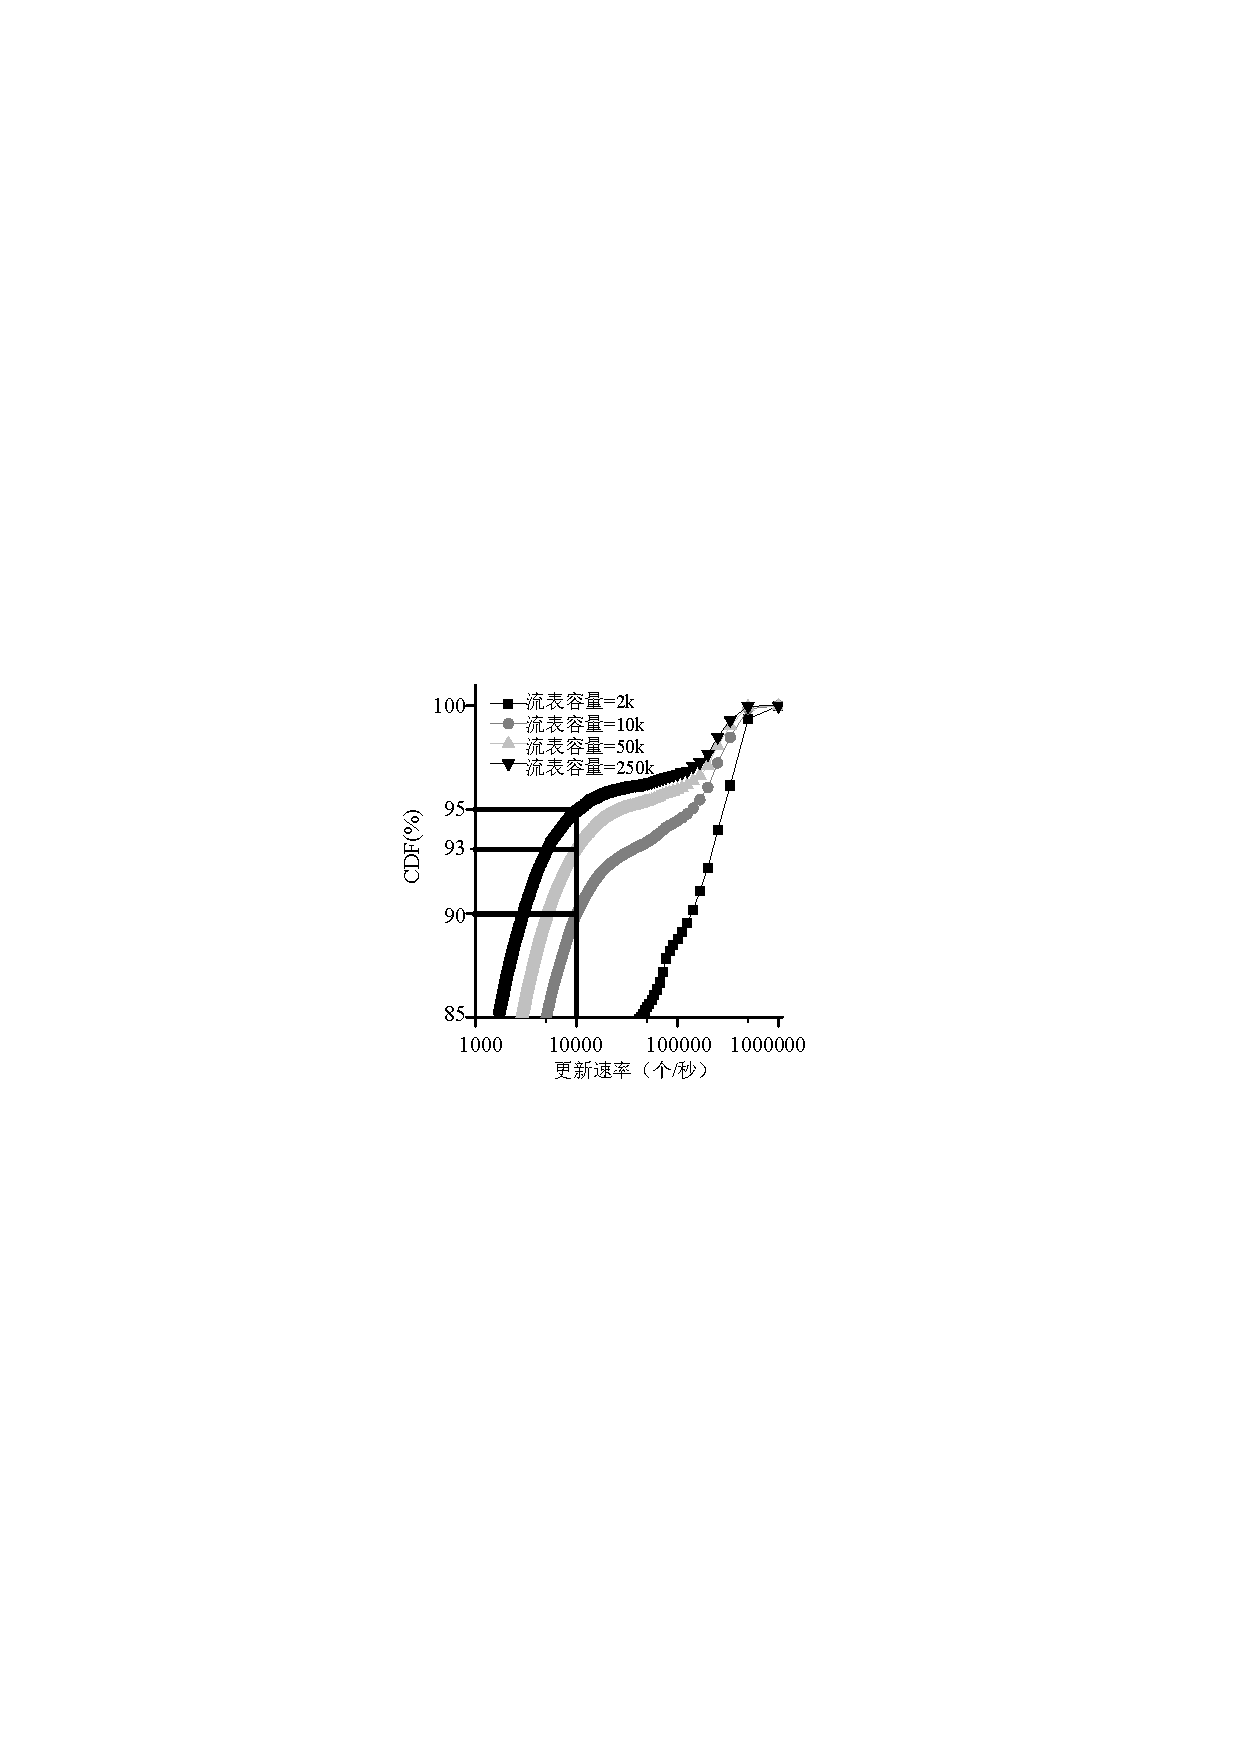
\includegraphics[scale=1]{ftsupdate.pdf}
	\caption{流量更新速率的概率累计分布} \label{fig:ftsupdate}
\end{figure}

根据Openf协议,流表最大支持45个域(144Bytes),流表资源消耗量大的情况在OpenFlow交换机中尤为凸显。面对上述问题,为使SDN的优势在广域网间应用,业界不得不使用以及购买性能更强价格更昂贵的交换机。在实际应用中,若交换机流表资源不足,对于最终无法更新的流,交换机会将他们按照Table-Miss策略处理。目前的控制策略大都会以Packet-In消息的方式上报给控制器。若Packet-In消息数目过多,会引起安全通道传输阻塞以及引发控制器处理阻塞,不但会引发控制器安全问题,且影响到其他服务,会加剧数据平面转发效率下降。

\BiSubsection{流量细粒度趋势}{Flow Fine-grained Trend}

SDN的核心功能抽象为控制平面向数据平面安装流表项,OpenFlow交换机对数据包的处理过程遵照流表项内容进行转发。基于TCAM的查找表具有高速,流聚合等优良特性,已经广泛使用在交换机中。然而TCAM芯片设计复杂,电路面积巨大,价格高昂(2500人民币/Mbits),功耗大(15瓦/Mbits)。因而交换机无法存储全部流量信息。

如今网络已不局限于best-effort服务理念,服务提供商和内容分发希望流量有区分地进行服务,以提供不同场景不同服务价格,赚取差异化后的最大利益。此外数据中心和蓬勃发展的虚拟云主机市场也对网络流量细粒度管理提出更多需求\citeup{li2012toward,benson2011microte,cerrato2014supporting}。尽管OpenFlow协议下流表资源消耗量更大,但市场依然期待让用户得到SDN有利技术。越来越多的实例也展示了SDN技术的强大魅力以及逐步扩大的影响范围。如何应对大规模部署后日益匮乏的流表项资源,以及解决流表溢出导致的性能极端下降,并且如何高效地利用全网有限资源是亟需解决的问题,也是本章探讨的主要内容。


\BiSubsection{问题分析}{Problem Analysis}\label{chap532}

SDN架构使得控制平面与数据平面在物理上分离,交换机与控制器之间通过专用线路建立连接,通常专用线路称作“安全通道”(Secure Channel)。数据平面的配置内容会直接影响到网络的行为,因此对于交换机的配置需要确保严格的安全性。OpenFlow协议利用各类消息定义为应用程序接口,数据和功能打包为数据包在安全通道内传递。SDN对网络的控制因为安全通道传输开销,导致系统控制延迟大于传统网络\citeup{curtis2011devoflow}。研究人员面对了两个源自于SDN架构的挑战:(1)控制平面---消息数量庞大,控制器一般较为复杂、性能要求极高;(2)数据平面---流表空间有限,流表溢出易造成性能大幅下降。

第一类问题,研究人员已经提出了分布式多控制器原理\citeup{koponen2010onix},专用子控制器\citeup{yu2010scalable},提升控制平面的性能方法。本文主要针对第二类问题,即对数据平面可扩展性问题进行研究,分析其可能造成的严重后果。目前OpenFlow交换机有两种实现架构,第一是软件交换机,第二是基于硬件的交换机。二者各有优势,软件交换机通常部署在服务器虚拟机环境内,软件交换机的流表项大多存储于内存空间。服务器内存空间资源通常比较丰富(多达上百GB),足以保存足够多的规则,拥有资源冗余度。软件交换机应用范围有限,主要适用于交换吞吐较低的场景(10Gbps以内)\citeup{katta2014infinite}。可将流量较小,流数目丰富的老鼠流交由软件交换机处理。但对于高性能场景(大于1Tbps),依然须使用基于硬件的OpenFlow交换机。

对网络领域进行行为分析,一般使用泊松过程。

\begin{theorem}%[Riesz 表示定理]
	假设数据包的到达服从参数为$\lambda$的泊松过程,$ Flow\_number(T) $为流数量随时间分布,则必然存在某一时刻,使得容量为$C$的流表充满。即存在某时刻$t$使得:
	
	\begin{equation}
	Flow\_number(T) \geq C, \qquad T \in (t,t+\Delta t)
	\end{equation}
	
\end{theorem}


\begin{proof}
	假设交换机中流表容量为C条,数据流的到达模式为具有参数$\lambda$的泊松过程,流的生存时间为服从速率参数$\mu$的指数分布,$N_t$为在$t$时刻流表中的流个数。显然,$N_t$是一个增消过程,若到达强度$\rho>1$,$N_t$将无边界增长。因而需满足:
	
	\begin{equation}
	(\rho=\dfrac{\lambda}{C\mu})<1
	\end{equation}
	
	$N_t$的稳态概率密度分布函数推导如下\citeup{kleinrock1975queueing,singlestation}:
	
	
	
	\begin{align}\label{fts1}
	&\pi_0 = [\sum_{k=0}^{C-1}\dfrac{(C\rho)^k}{k!}+\dfrac{(C\rho)^C}{C!}\cdot\dfrac{1}{1-\rho}]^{-1}  \\
	&\pi_k = \begin{cases}\label{fts2}
	\pi_0\dfrac{(C\rho)^k}{k!}, \qquad 0<k<C \\
	\pi_0\dfrac{\rho^kC^C}{C!}, \qquad C \leq k
	\end{cases}
	\end{align}
	
	其中$\pi_k$代表流表中已经有$k(=Flow\_number(T))$个流表项的概率。
	参考爱尔兰公式\citeup{kleinrock1975queueing},流表充满的概率为$ P(C\geq  k) $:
	
	\begin{align}\label{fts3}
	P(C\geq  k) &= P(C,\lambda/\mu) \nonumber \\
	&=\dfrac {\left( \dfrac {\left( C\rho\right)^C}{C!}\right) \left( \dfrac {1}{1-\rho }\right) }{\sum ^{C-1}_{k=0}\dfrac {\left( C\rho\right) ^{k}}{k!}+\dfrac {\left( C\rho\right) ^{C}}{C!}\cdot\dfrac {1}{1-\rho }} \nonumber  \\
	&=\dfrac {1}{1+\left( 1-\rho \right) \left( \dfrac {C!}{(C\rho)^{C}}\right) \sum ^{C-1}_{k=0}\dfrac {(C\rho)^{k}}{k!}}
	\end{align}	
	
	由公式\ref{fts2}中$ k $超过$ C $时的概率密度函数,以及公式\ref{fts3},显然不论$ \rho $、$ C $、$\mu$取何值,总有概率$ P(C,\lambda/\mu) $ ,使得$ Flow\_number(T) \geq C $。
\end{proof}

\begin{figure}[!ht]
	\vspace{-1.5mm}
	\centering 
	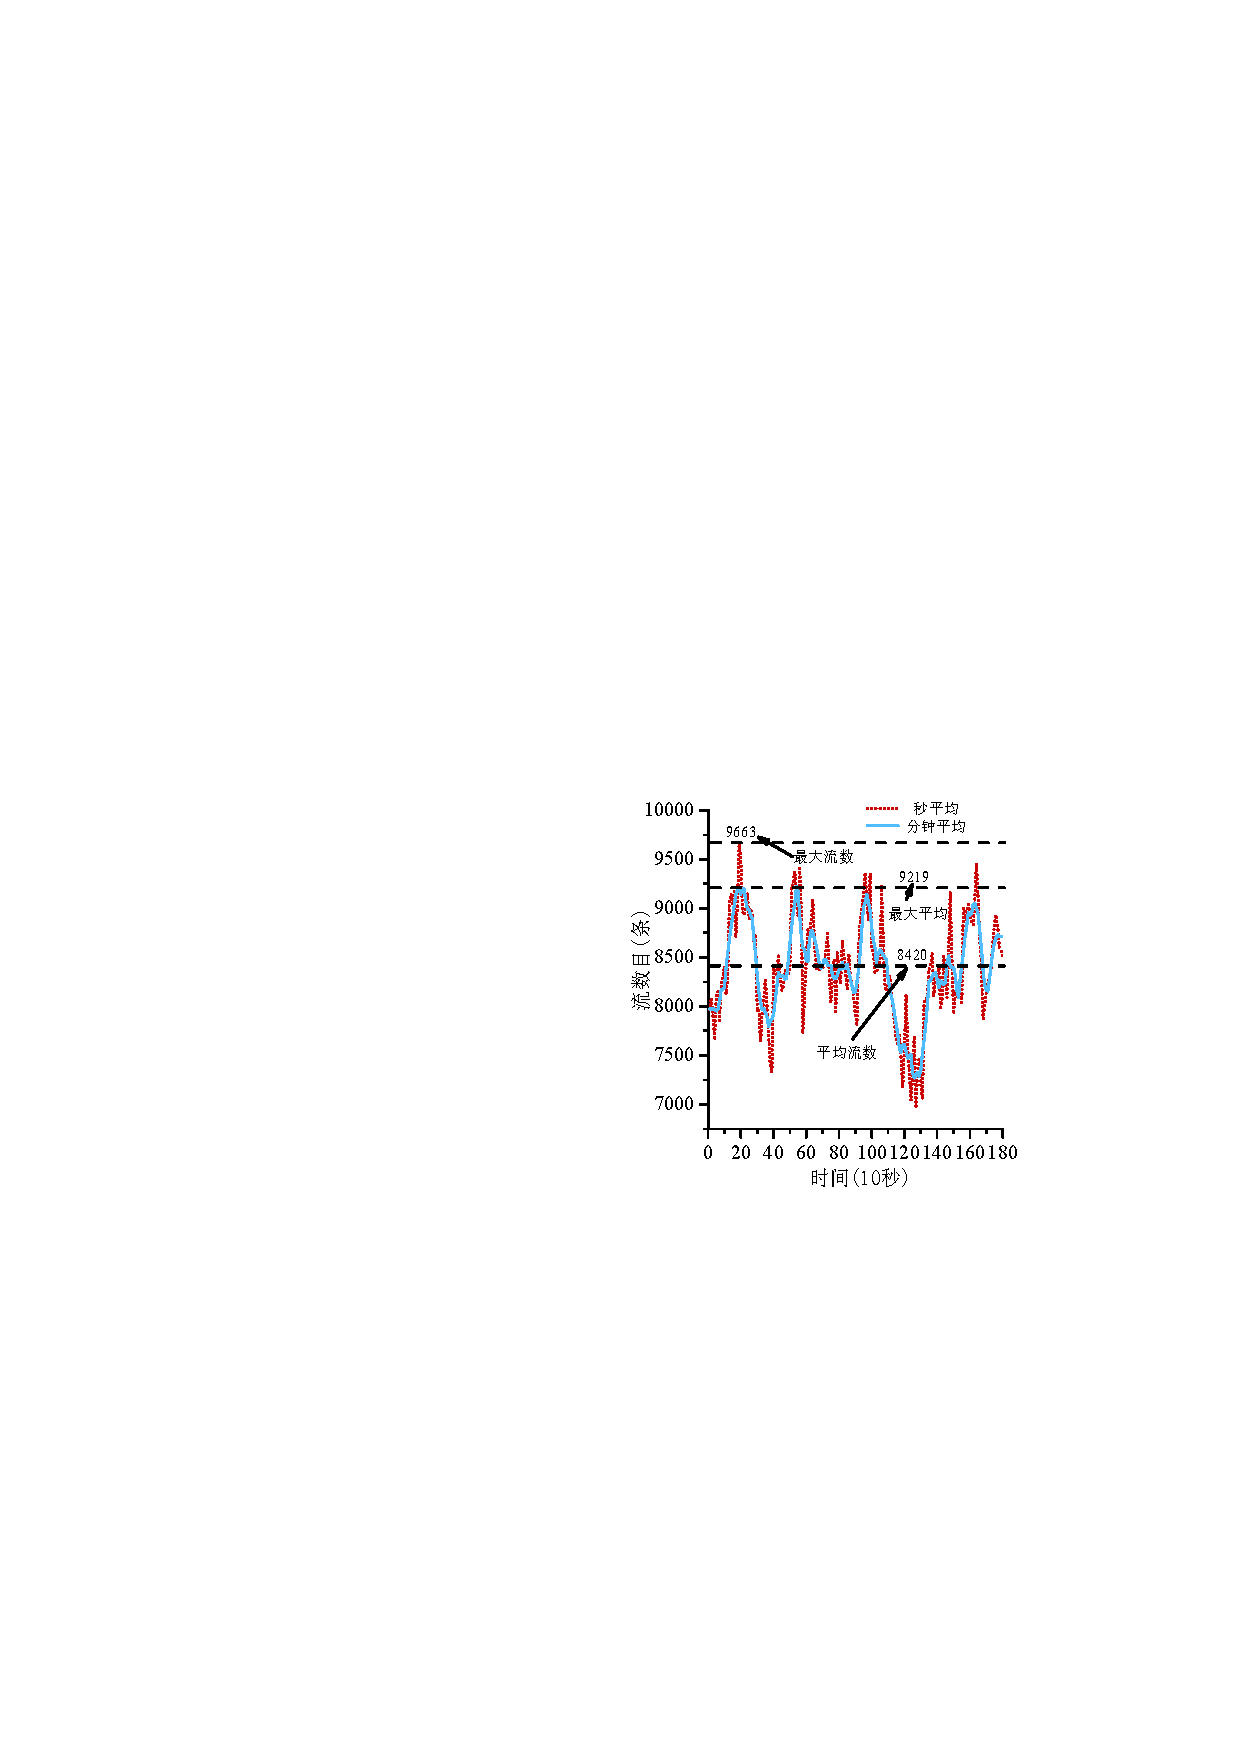
\includegraphics[scale=1]{ftsbigflow.pdf}
	\caption{以10秒为窗口统计流数目} \label{fig:ftsbigflow}
\end{figure}

为得到真实流量特征的统计,本文对广域网(ISP)流量\citeup{allesina2004wand}样例进行了分析,并截取如图\ref{fig:ftsbigflow}所示30分钟时间内流数目情况(流分类取前16bit目的IP地址)。可以发现,平均流数目为Avr=8420,假设控制器没分钟对全网流量(削峰填谷)实施调度,则最大流表容量需求为Max\_Avr=9120条。然而在极短暂时刻同时($t+\Delta t$)最多有k=9663条流同时到达交换机。因此可以计算出流数目超过Max\_Avr的概率为8.9\%,剩下91.1\%的时间内,交换机中有7.6\%的流表是空闲的。网络开发人员应根据已有设备的流表资源来决定调度策略的最大精细程度。根据流表使用比例动态调整流表项分布策略是可行的。为保证应用尽用,使经济效益最大化,则有约束条件:

\begin{equation}\label{fts4}
C \leq Max\_Avr \leq k 
\end{equation}

\begin{equation}\label{fts5}
Avr \leq C 
\end{equation}

\ref{fts4}表示容量C若小于最大平均值Max\_Avr有助于提高流表资源平均使用率。公式\ref{fts5}保证流表不可被时时刻刻充满的冗余性条件,因此实际平均使用数目须小于C。在上述两公式的条件下,全局资源中一定有过多的冗余,本文希望减小全网的流表空间浪费率。

数据平面发生流表溢出的概率始终存在,下面分析流表溢出现象对网络通信服务造成的性能危害。OpenFlow1.3协议规定,当控制器准备向交换机下发流表项时,若交换机流表已经被装满,其会向控制器发送错误报告<ofp\_error\_msg,OFPFMFC\_TABLE\_FULL>,并且交换机端会拒绝安装这条流表项。控制器得到错误返回后, 可以选择忽视这条新流,也可以执行流表替换。若:1)忽视此流,则会造成拒绝服务现象;2)控制器服务此流,则需先删除某条已有规则,再重新添加此流表项。但如果被删除的已有流表项是活跃流,继而又会造成活跃流中断服务。因此会有可能导致数据包传输延迟增大,传输速率降低,发生丢包现象。本章将在\ref{chapftsevaluation}章测试流表溢出后通信效果的变化。



\begin{figure}[!ht]
	\centering 
	\vspace{-1.5mm} 
	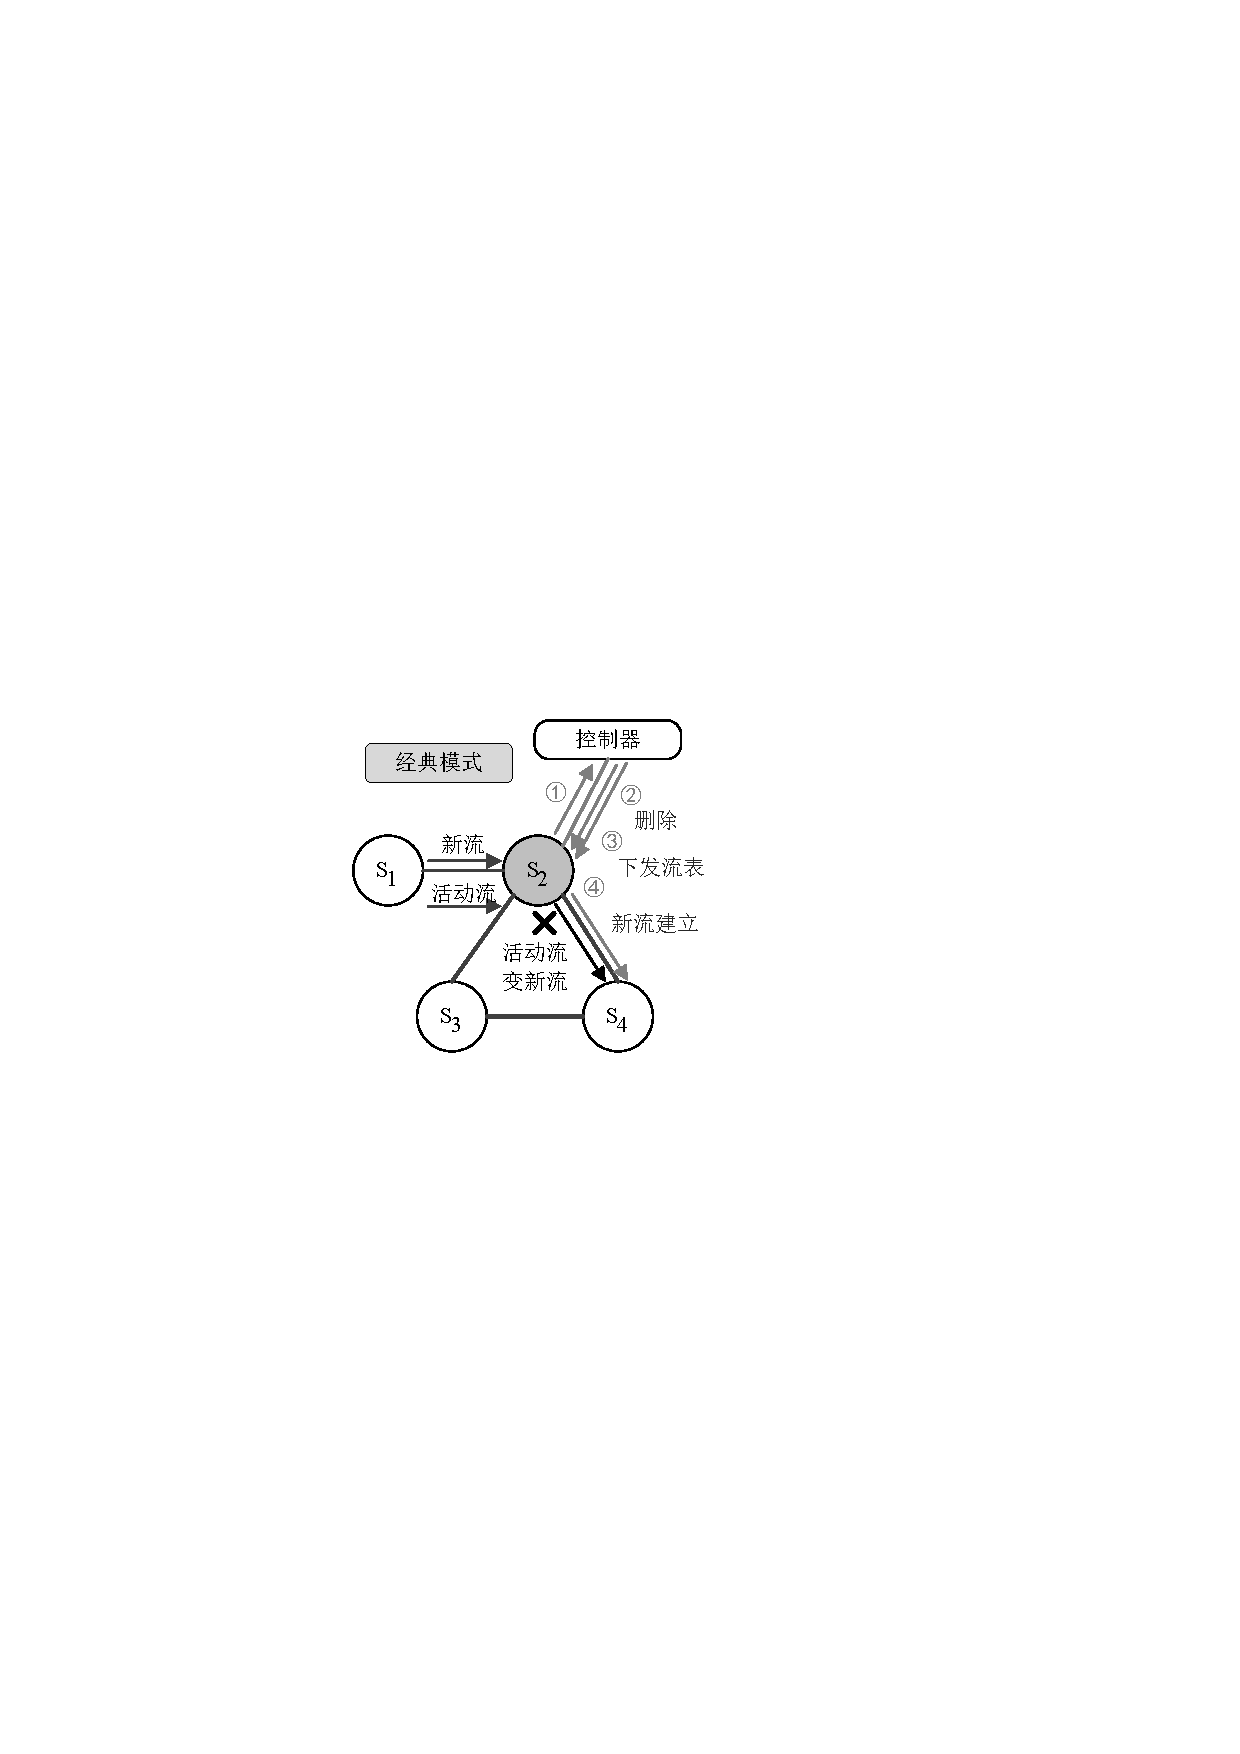
\includegraphics[scale=1]{ftsnewflow.pdf}
	\caption{OpenFlow协议新流处理过程} \label{fig:ftsnewflow}
\end{figure}

下面本文以一个实例具体分析以上论述,图\ref{fig:ftsnewflow}所示为交换机组成的简单拓扑。每交换节点都与控制器相连。假设在某时刻,S2交换机内流表容量空间被填充满。之后如果再有新流到达,按照目前OpenFlow协议并对S2交换机分析系统操作流程:(1)S2交换机查找表项未匹配,并触发Packet-In消息;(2)控制器接收Table-Miss消息后下发新表项,并且控制器S2流表发现已经溢出,选择某条流表项删除;(3)控制器下发新流到S2;(4)对新流转发建立成功。



由于控制器删除的原有流有可能是某活动流(active flow),并未超时退出,此流接续数据包会快速到来。然而控制器无法轻易获取数据平面内哪条流是最长时间没有到达的,控制器无法按照最优方式删除活动流。在流表项被删除后,后续数据包会被交换机重新判别为新流。网络控制闭环将循环重复前面的过程。新流频繁到达会导致大量重复控制消息数据包充斥在安全通道内,大量耗费控制器的计算处理资源,且占用安全通道有限通信带宽,同时使交换机服务新流量效率低下。
另外一种解决办法:控制器发现流表空间存储已满,不向交换机内替换新流表项。这样虽然保证了已有流量正常转发,但会导致系统放弃对新流的响应。综上,本文面对问题最根本原因是由于流量大小起伏波动,流数量暂时超过交换机容量上线,导致单点转发性能下降,进而影响整体网络服务质量。




\BiSection{流表共享机制}{Flow table Sharing Mechanism}\label{chap54}

针对之前两小结节所提出的问题,本文提出了一种全局流表共享机制(Flow Table Sharing, FTS),该机制目标为缓解由于流表溢出造成交换机转发能力下降以及暂时无法提供服务的现象。FTS机制实现两个关键特性优化:1)允许流表溢出时交换机转发新流;2)减小安全通道内重复控制消息的数量。

\BiSubsection{允许流表溢出时交换机转发新流}{Allow the Switch to Forward New Flows When the Flow Table Overflows}\label{chap541}


挑战1:没有建立流表项的流无法执行转发动作。在经典的<匹配-执行>操作方式,数据包在被匹配成功之后方能得到正确处理。当交换机内没有足够流表空间,针对新流匹配表项无法安装。交换机不会对新流执行任何操作。但本文希望当交换机无对应流表项时允许转发,这与目前模式相矛盾。

解决方案:为交换机增加随机转发特性。与<匹配-执行>不同,随机转发只将流量转发到邻居节点。这种方式没有精确的策略指导,转发出口只要不等于入端口即可(避免路由环路的产生)。因此这条本被拒绝服务的流,出现在邻居节点内。由于邻居节点与本地节点同时发生溢出的概率很小,这条流会有更大的几率成功地在邻居节点上建立流表项。



\BiSubsection{减小重复控制消息的数量}{Reducing the Number of Repeated Control Messages}\label{chap542}

挑战2:由于新流频繁到来,会引发重复的Packet-In消息。在OpenFlow协议下,交换机收到无匹配规则的流后,会触发Packet-In消息机制。Packet-In消息携带包头信息给控制器,控制器依据此判断处理方法。当流数量超过流表容量时,对交换机而言当前时段内无法处理的数据包都可归为新流。将导致带有相同包信息的控制消息在安全通道内反复传递,占用有效控制信息通信带宽。

解决方案:本文将通配转发引入随机转发模式内。因此对于任意一条无法处理的新流,都会匹配执行。交换机总能保证数据包被处理,从而避免产生重复的Packet-In机制。下一节详细论述FTS结构的设计与实现。



\BiSection{基于OpenFlow交换机的随机路由策略}{Random Routing Strategy Based on OpenFlow Switch}\label{chap55}

为抑制在流表溢出时更新流表而产生的重复控制消息,改善由于新流没有相应<匹配-执行>而信息无法获被转发的现象,本文提出一种<随机转发-流表扩散>方法。流表溢出的节点利用邻居节点内的空闲资源,重新建立从邻居到目的地的转发路径线。

为保证此机制可正常运作,显然如果网络中所有交换节点均可随机转发,必然引起数据风暴或无正确路径。因此假设网络中流表溢出只会发生在随机的少量的节点内。可以利用反证法证明:若网络内大部分结点都存在流表溢出,此情境下的网络必处于大面积拥塞的状态。但从实际观察,绝大多数时段内网络并不会出现大规模拥塞。网络内流表总有足够的冗余度,能满足基本的流量波动。另外,控制器也会实时根据拥塞情况调整网络流量控制粒度。因而流表项的平均使用率只会趋于最大用量,从宏观角度保障不会普遍溢出。



\begin{figure}[!ht]
	\centering 
	\vspace{-1.5mm} 
	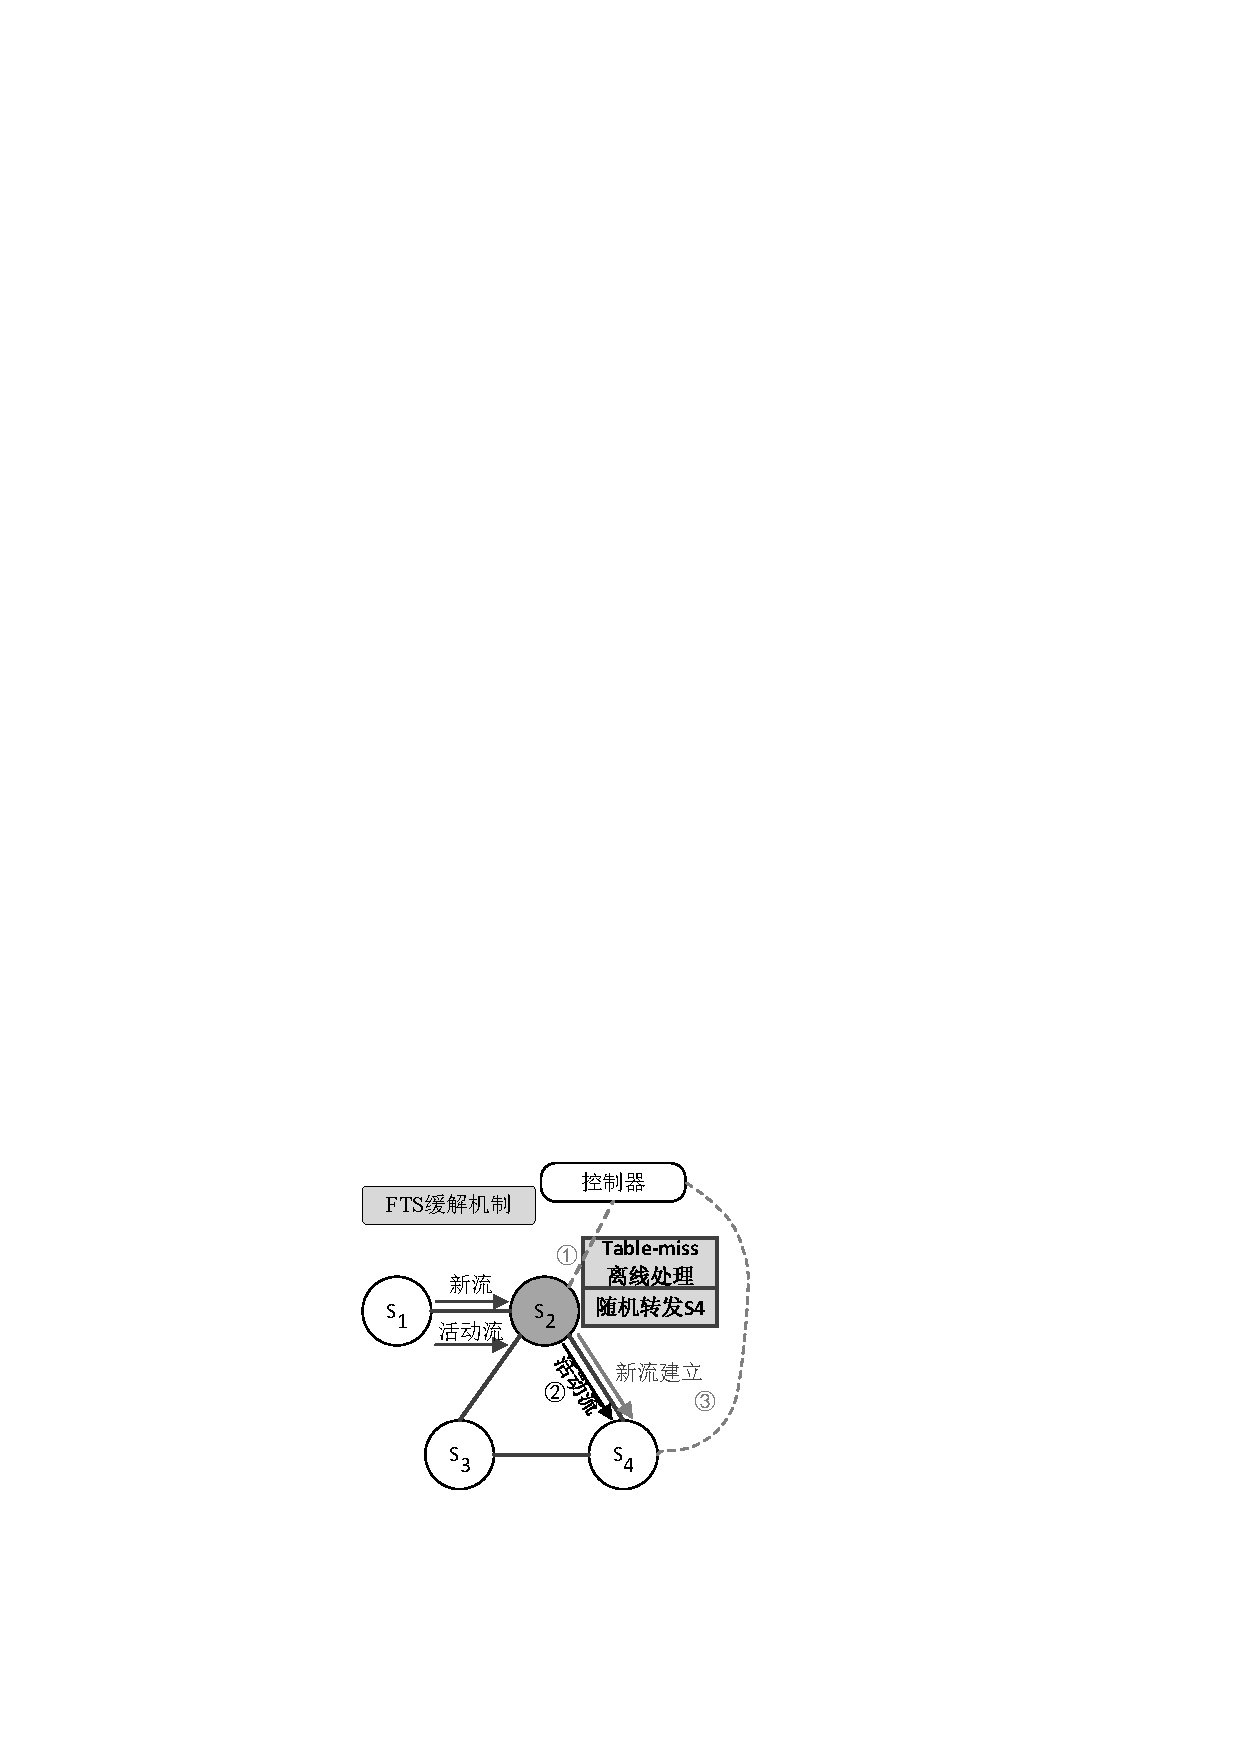
\includegraphics[scale=1]{ftsfts.pdf}
	\caption{流表溢出后FTS对新流的处理流程} \label{fig:ftsfts}
\end{figure}

图\ref{fig:ftsfts}展示了本文提出的FTS机制新流的处理方式。假设当交换机S2流表溢出,且此时新流到达并匹配为Table-Miss,交换机不产生Packet-In消息。(1)交换机流表溢出时,只在本地执行离线策略。通过一定的快速本地计算,得到新流相应的转发动作,从而避免丢弃数据包。其中的快速随机转发,应满足线速需求。(2)在本例中,新流被转发到S4中,且之前建立的活跃流不会受到本地策略的影响,可以持续转发。(3)新流到达S4后,在此邻居节点上重新部署路由。下面的两小节详细说明交换机离线策略及实现方式。

\BiSubsection{随机路由离线策略设计}{Random Routing Offline Strategy design}



本文将交换机中离线随机策略抽象为下图\ref{fig:ftsppl}中的形式:

\begin{figure}[!ht]
	\vspace{-1.5mm}
	\centering 
	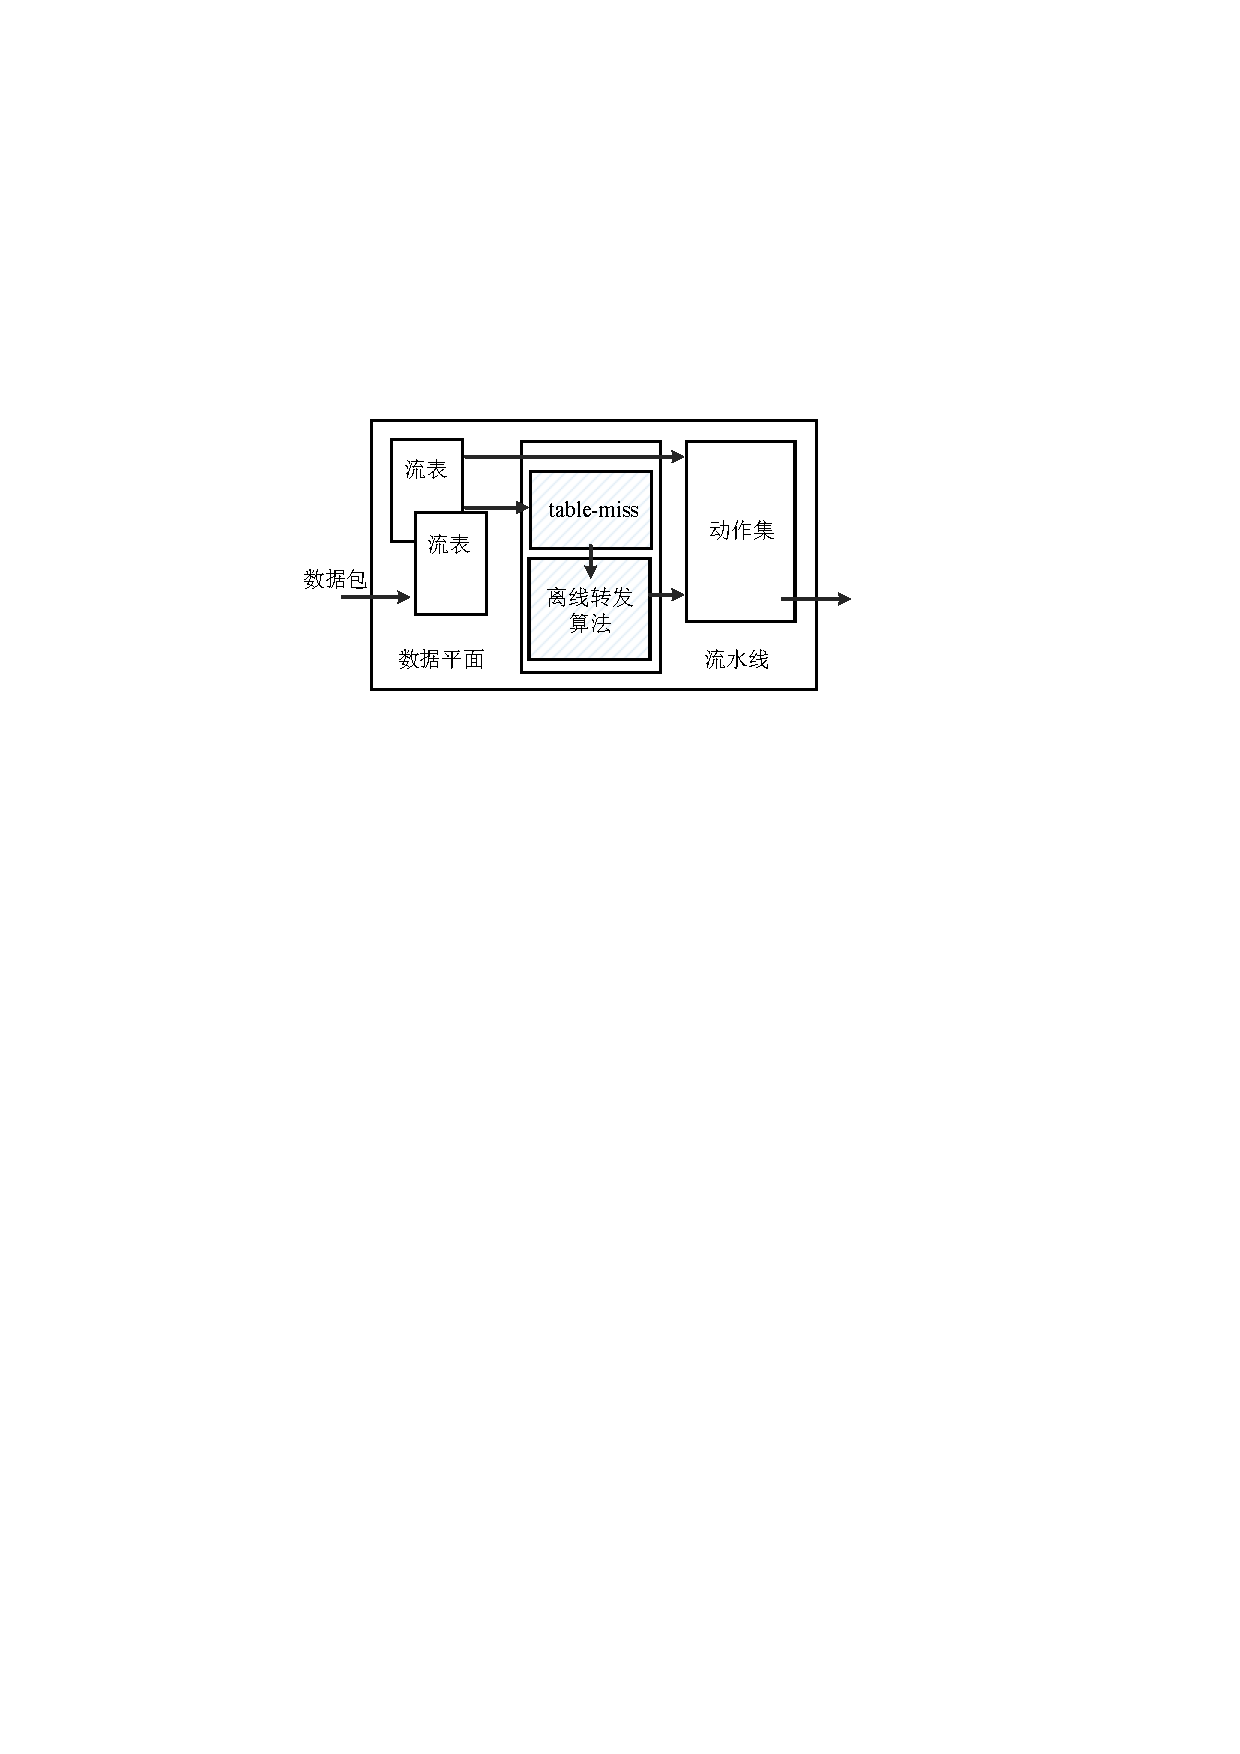
\includegraphics[scale=1]{ftsppl.pdf}
	\caption{FTS目标交换机的流水线结构} \label{fig:ftsppl}
\end{figure}


数据包到达交换后机首先执行流表查找,匹配成功后执行已配置的处理操作:例如,计数器更新,指令集执行等。而后判断流表是否处于溢出状态且是否需要触发Table-Miss事件。如果没有溢出则直接执行动作集,此处动作集包括触发Packet-In消息;若流表溢出,则在本地计算数据包的发出端口。%%%%%%%%%%%%%%%%%%%%%%%%%%2020年7月24日12:25:49 qsy
包含FTS机制的交换机与OpenFlow交换机的区别仅体现在增加触发Table-Miss事件时,判断交换机是否发生流表溢出;以及在本地离线处理策略内out\_port端口计算方法。为支持线速转发,上述算法只能在交换机硬件快速流水线中实施。修改交换机硬件流水线难度较大,但考虑到流水线内的组表,指令集,动作集都等可以灵活配置。因此本文须解决将此算法与OpenFlow交换机流水线内拥有可重配特性的组件耦合起来。
将本文总体设计总结如下:
1.流表匹配。经过流表匹配后,得到packet是否为Table-Miss。 
2.根据metadata以及交换机本地判断提供的流表空间使用率,判断是否需要离线计算。
3.流水线中out\_port的算法计算数据包的发出端口。
4.执行动作集。
其中必须满足的限制条件:
1.随机转发的出端口(out\_port)不可等于入端口(in\_port),否则产生环路。
2.为满足吞吐速率,out\_port随机算法须简洁高效。
限制条件带来以下2个硬件实实现上的挑战:
1.随机方法。无现成的指令集为随机指定动作集。
2.以目前OpenFlow协议实例的硬件流水线无溢出判断。贸然修改交换机流水线不符合OpenFlow标准的协议,会导致交换机兼容性性差的缺点。
本文为应对以上的挑战,选择以组表作为OpenFlow交换机实现随机转发的关键部件。



\BiSubsection{随机路由策略组表方式实现}{Random routing strategy group table implementation}

1)OpenFlow组表。

OpenFlow协议规定组表(Group-Table)属于交换机流水线内固定功能,组表是多个动作桶的集合(Action Buckets)。每一个动作桶包括一组可执行动作集和相关参数。组表类型有:ALL, SELECT, INDIRECT, FAST FAILOVER,四种。本文选择组表的SELECT操作类型。
SELECT(选择算法):一个数据包只选定组内的一个桶执行,选取逻辑由用户选择算法指定。例如哈希某些数据包头域,或者基于Round-Robin选择。OpenFlow协议不限定选择算法种类。

\begin{figure}[!ht]
	\centering 
	\vspace{-1.5mm} 
	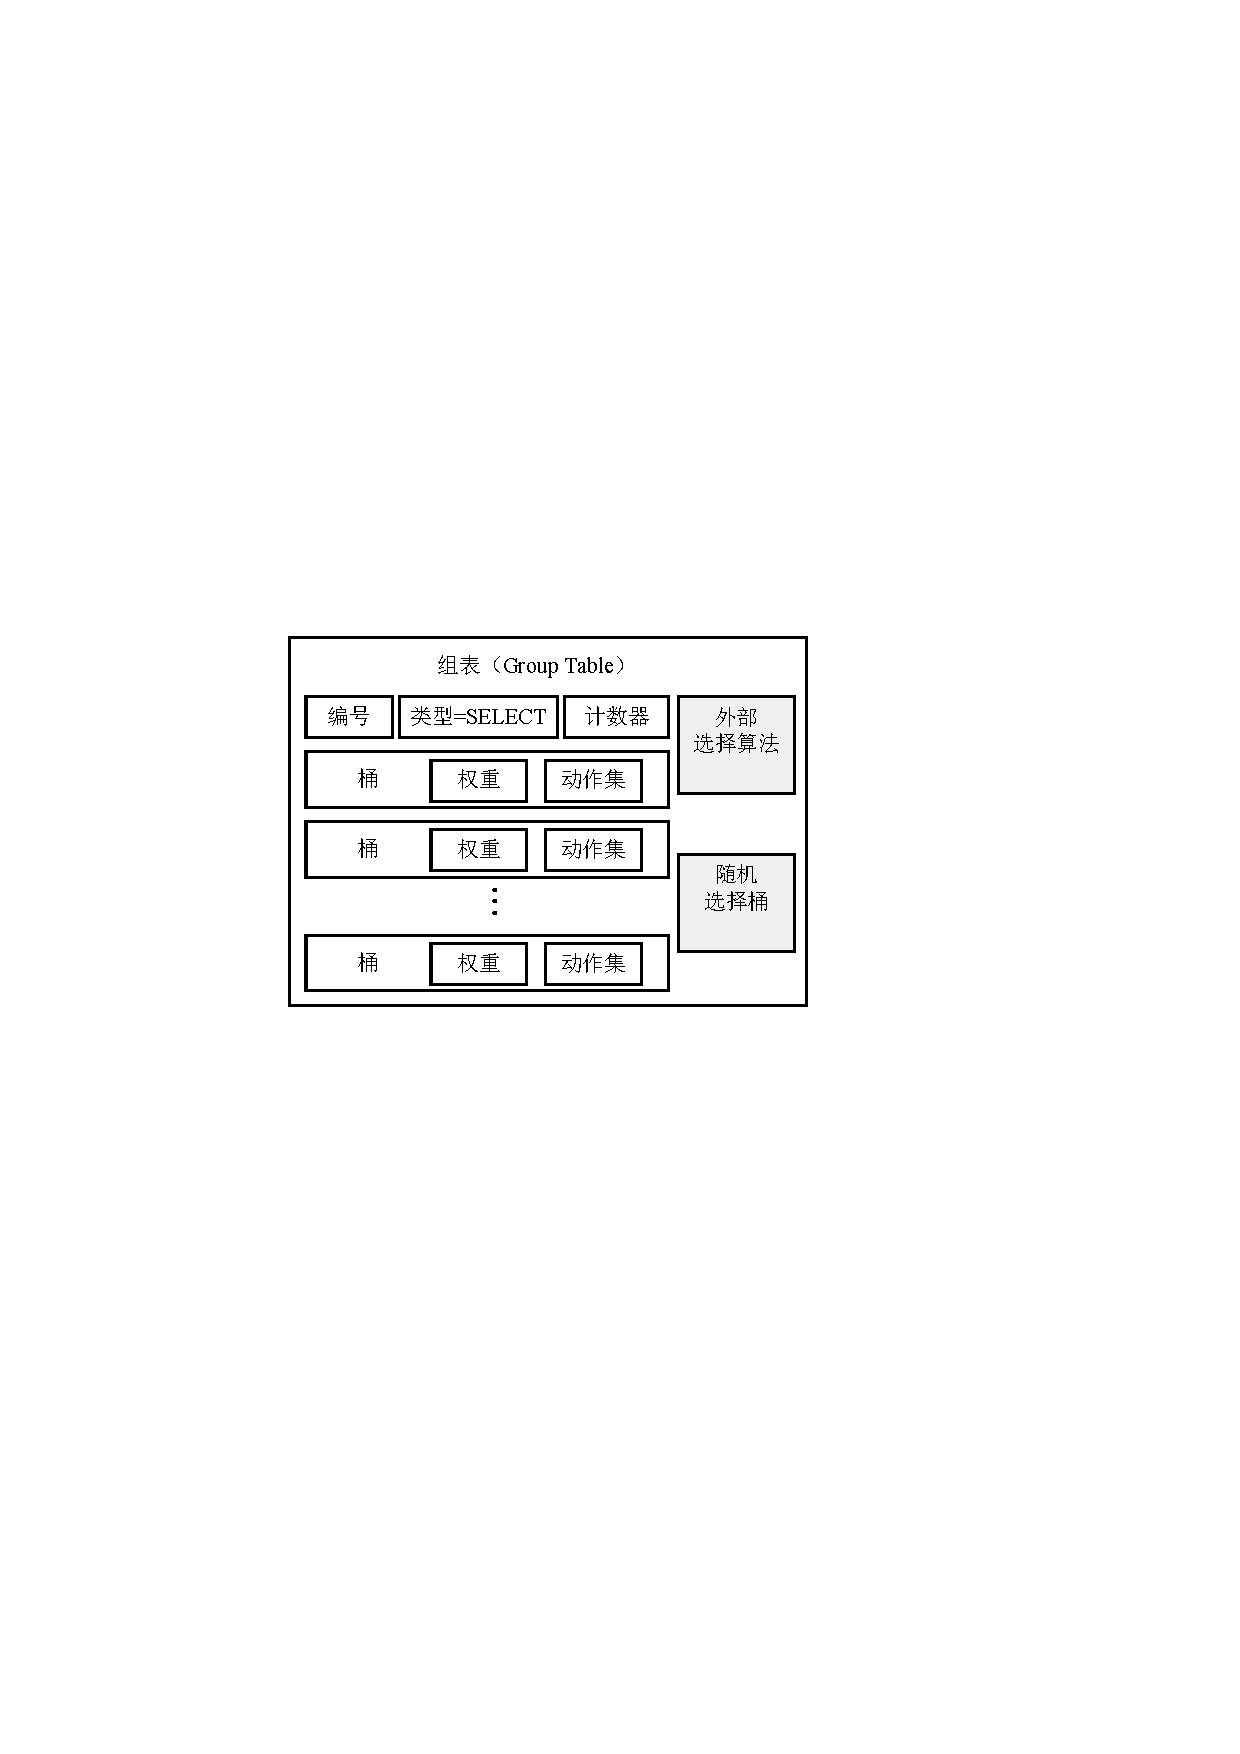
\includegraphics[scale=1]{ftsgp.pdf}
	\caption{OpenFlow组表结构} \label{fig:ftsgp}
\end{figure}

如图\ref{fig:ftsgp}所示,组表数据流水线内动作集的一部分。组表将多个动作集内容通过算法融合到一起,给数据包带来更灵活的操作。组表内包括编号字段、组表类型、计数器和桶。不同的组表类型中桶的执行方式也不同。OpenFlow协议下组表的SELECT可以由终端用户自行定义,此选择算法用来从所有桶中选择一个执行,若属某一个选定的桶动作集输出端口失效,逻辑应自动将桶待选范围缩小至剩余可用桶并重新做选择。

某些选择算法已经标准化在硬件组表内,例如,使用哈希算法分类用户配置的包头数据域,或简单的令牌环。本文使用OpenFlow组表解决了前文提出的两个挑战,利用随机选择桶算法实现随机,组表天然的又是硬件流水线内的一部分,能够满足线速转发的要求。

下一小节讨论:根据本文提出的组表方案,应该如何设置流表以及组表:(1)出端口不能等于入端口,(2)流水线随机算法应简洁高效。


2)组表桶的设定。

数据包转发出口由桶内的动作集用指定,权重表示此桶被选概率的大小。要求向邻居节点随机转发,则桶内的动作集内转发出口(out\_port)的值应该对应自己本机的邻居节点。显然,数据包出端口不会包括入端。可选择两种方案解决:(1)结合流表进行二级匹配,区分并剔除源端口;(2)开发额外组表选择算法剔除入端口。

\begin{algorithm}[!h]
	\caption{组表外部选择算法 \label{ftsa}}
	\IncMargin{2em}
	\DontPrintSemicolon
	
	\KwIn{in\_port}
	\KwOut{out\_port}
	
	\While{New packet arrival}{
		\If{Not overflow}{out\_port = CONTROLLER}
		\Else {
			out\_port=(out\_port+1) mod $ N $
			
			\If{out\_port == in\_port}{
				out\_port=(out\_port+1) mod $ N $
			}
		}
	}
	\Return out\_port
	
\end{algorithm}

(1)结合流表二级匹配。流表项的匹配域为in\_port,设置对应组表的group\_id = in\_port 。此组表内的桶不含转发到PORT=in\_port的动作集。之后由令牌环算法实现简单高效的随机动作。需要将此流表项配置成最低优先级,以保证此流无其他流表项可匹配。例如,交换机有N个邻居,则需要在流表内添加$ N $条表项,再配置相应的$ N $个组表,每个组表内包含N-1个buckets;空间复杂度为$O(N^2)$。另外须考虑流表溢出的判断:第一,本文可利用控制器监控流表使用情况,一旦溢出发生,控制器再向交换机内填写$ N $个扩散流表项,但是这会造成较大控制延迟。第二,可以利用外部选择算法,在交换机内部判断,控制器须将$ N $个扩散流表初始化到交换机内。

(2)采用额外组表选择算法。扩充组表内的选择算法,则只需要使用一个组表,组表内动作集包括向所有的N个邻居、和1个控制器(CONTROLLER)端口转发。若算法判断交换机流表没发生溢出,直接选择转发向CONTROLLER的端口。在溢出的情况下,out\_port选择算法结果需要同in\_port做比较。随机算法可以用简单令牌环实现,一旦发现out\_port与in\_port相同则选择下一个桶直接执行即可。
方法总结1:空间复杂度大:其中流表占用$O(N)$、组表占用$O(N^2)$;初始化复杂,但是无需用户修改组表内的固定的选择算法。
方法总结2:空间复杂度低:流表占用$O(1)$,组表占用$O(N)$,初始化无延迟,但是需要自行开发组表内的选择算法。
由于OpenFlow协议对于SELECT算法并无强加限制,允许SELECT算法由交换机自行构成。因此本文更倾向于使用第二种方案,制定一种可扩展性强的SELECT算法(\ref{ftsa})。



\begin{figure}[!ht]
	\centering 
	\vspace{-1.5mm} 
	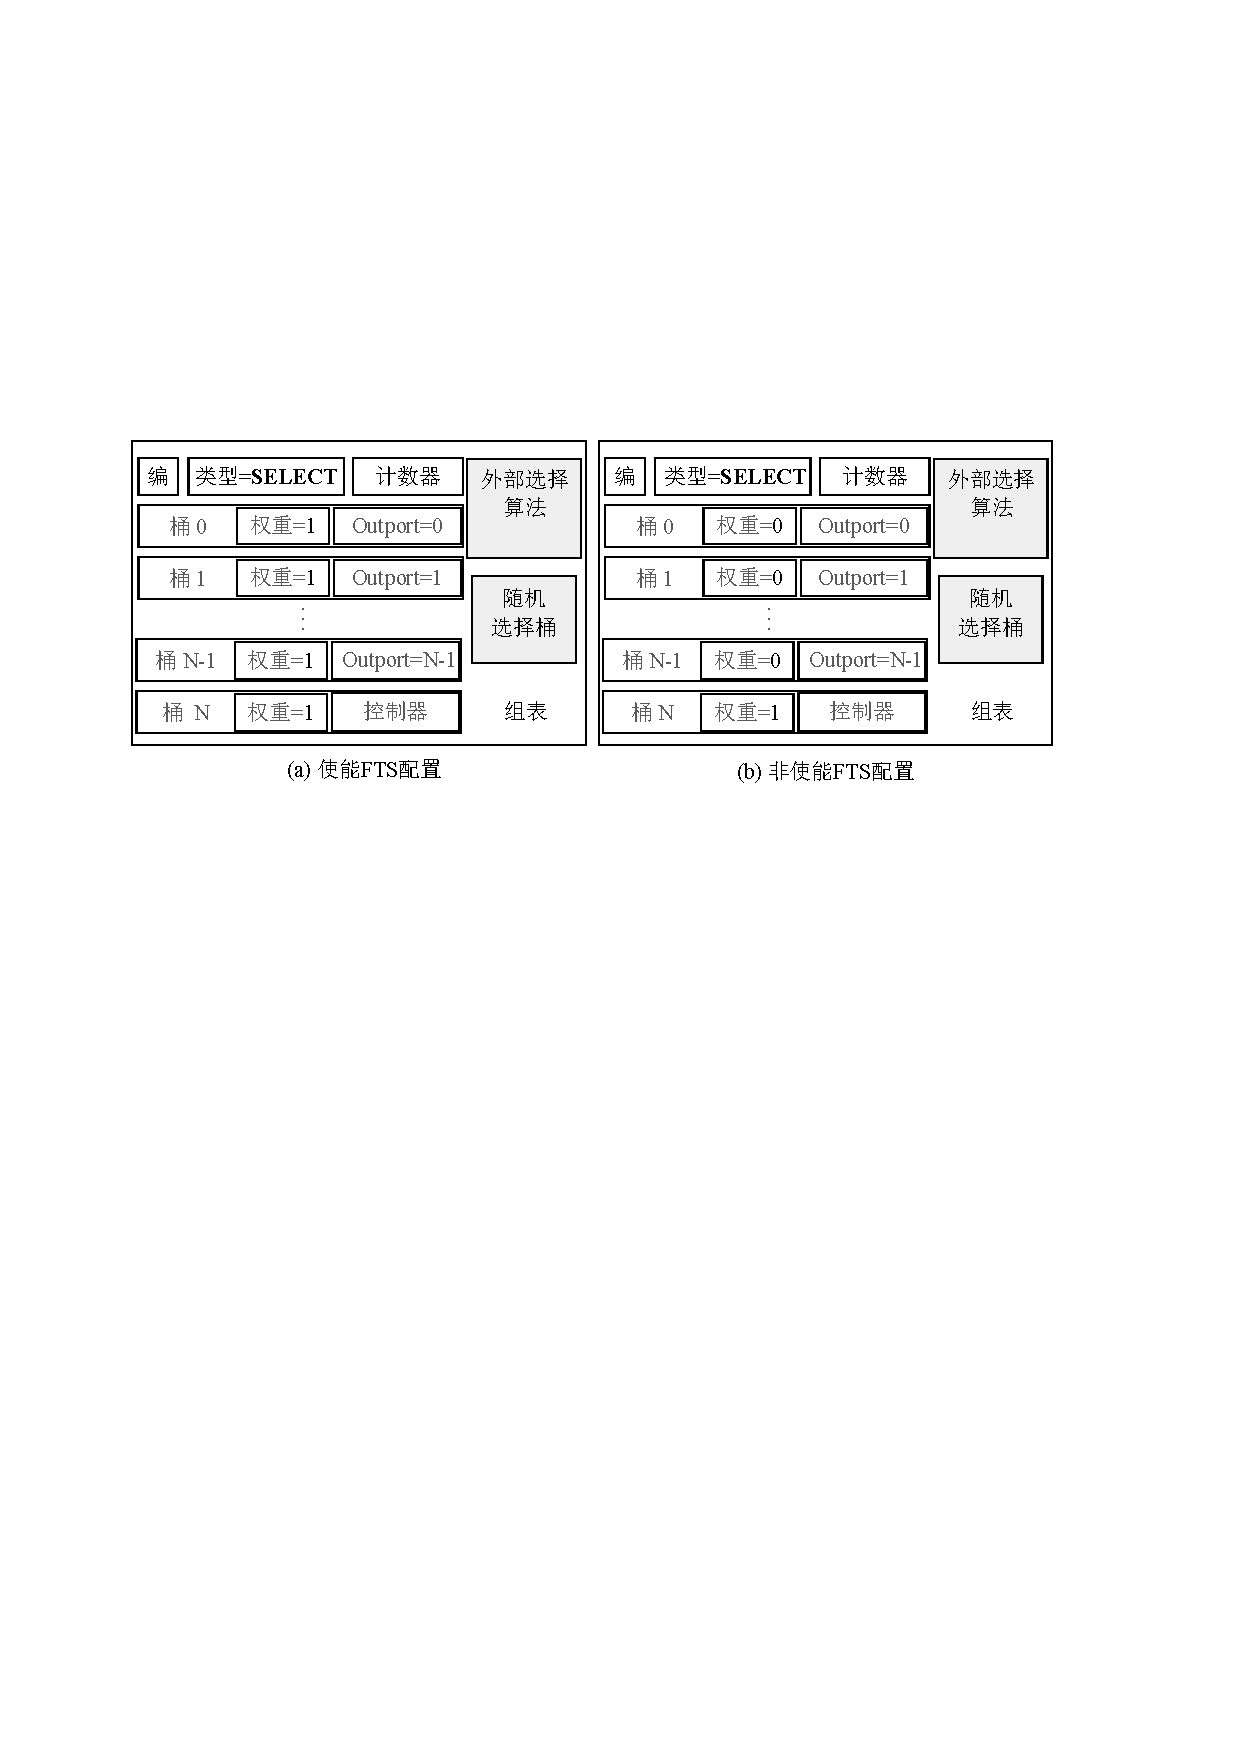
\includegraphics[scale=1]{ftsgpfts.pdf}
	\caption{组表的配置方式对比} \label{fig:ftsgpfts}
\end{figure}

如图\ref{fig:ftsgpfts}(a)所示,方形框内表示OpenFlow协议所规定的组表结构,包括了1.组表编号,2.类型,3.组表计数器,4.一个(或多个)桶,5.随机选择算法,6.外部选择算法。默认的随机选择算法是基于硬件的令牌环算法。

如图\ref{fig:ftsgpfts}(b)所示,从逻辑上外部选择算法是Table-Miss处理的延伸。因为桶内的权重可被设为1,表示可被作为out-port的候选对象。若bucket.weight= 0,选择算法会将此bucket对应的桶屏蔽。若所有bucket的权重都为0,此数据包会被丢弃。所以目前Table-Miss的处理方式可以由组表转换表达。取消应用扩散算法也比较简单,只要将前$ N $个buckets的权重设置为0即可。或者设置某些bucket的权重为0,即可屏蔽向对应邻居扩散的通路。





\BiSection{系统评估}{Evaluation}\label{chapftsevaluation}

实验测试包含2个部分,分别为:(1)使用软件仿真,对比FTS与优化之前转发性能优劣。(2)在真实拓扑中测试流表共享机制的部署开销。

第一部分转发性能测试实验使用了软件仿真平台,由于其仿真性能与硬件转发设备有很大差距,因而本文首先主要针对转发时延,讨论软件仿真实验的系统误差。记:当流表溢出后的流量总时延为$T_{over\_flow}$,FTS优化后的流量时延为$T_{FTS}$,单个数据包转发时延$T_{fwd}$,单个数据包传输时延$T_{trans}$,传输时延统计误差$\Delta T_{trans}$,转发时延统计误差$\Delta T_{fwd}$。因控制器与交换机都实例化在同一台计算机系统内,因此数据包的传输时会将远小于真实值$T_{real\_trans}$:

\begin{equation}\label{fts7}
T_{real\_trans} = T_{trans} + \Delta T_{trans}
\end{equation}

实验的系统误差($\zeta$)主要来自于转发时延,和传输时延的测量:

\begin{equation}\label{fts8}
\zeta_{time} \propto \Delta T_{trans} + \Delta T_{fwd}
\end{equation}

软件交换机通常状况下转发延迟小于0.2ms,使用真实硬件测试转发时延则会远远小于0.2ms,因此:

\begin{equation}\label{fts9}
\zeta_{time} T_{fwd} \propto 10^{-1}ms
\end{equation}

一般对于一条远程TCP链接数据流的包传输延迟,可估计在100ms的数量级,因此:

\begin{equation}\label{fts10}
T_{trans} \propto 10^{2}ms
\end{equation}

实验总时延$ T $由转发时延和传输时延组成:

\begin{equation}\label{fts11}
T_{real\_trans} \propto T_{fwd} + T_{trans}
\end{equation}

真实的总时延$T$由实验得到$T$与误差组成,并且依据公式\ref{fts7}至公式\ref{fts11}可得到真实时延$T$与时延结果$ T(exp) $的关系:


\begin{align}\label{fts12}
T_{over\_flow} &\propto T_{fwd} - \Delta T_{trans} + T_{trans} + \Delta T_{trans}  \nonumber \\
&=T_{overflow}(exp) + 99.9ms
\end{align}


\begin{align}\label{fts13}
T_{FTS} &\propto T_{fwd} - \Delta T_{fwd} + T_{trans} \nonumber \\
&=T_{FTS}(exp) - 0.1ms
\end{align}

对于公式\ref{fts12}与\ref{fts13},可以得到结论:(1)引入测量值的误差后,溢出时的总时延高于其他值两个数量级以上,且误差不引起自身测量值数量级(均为$10^2ms$数量级)的变化。(2)由于时延误差$10^{-1}ms $远小于$ 7.56ms$的测量结果,因此误差可以忽略,因而FTS优化后的真实值也达到对其他两个数据的数量级差距。所以证明性能测试实验使用软件仿真是具有代表性的,能保证结果的准确度。此外对于性能测试实验,制作真实硬件交换机造价昂贵,不易配置导致实验手段缺乏灵活性,此番论证后从理论上显著降低了实验的困难程度,易于其他科研工作者进行重复验证。

\BiSubsection{性能测试:转发时延与控制消息数量}{Performance Evaluation}

\begin{figure}[!ht]
	\centering 
	\vspace{-1.5mm} 
	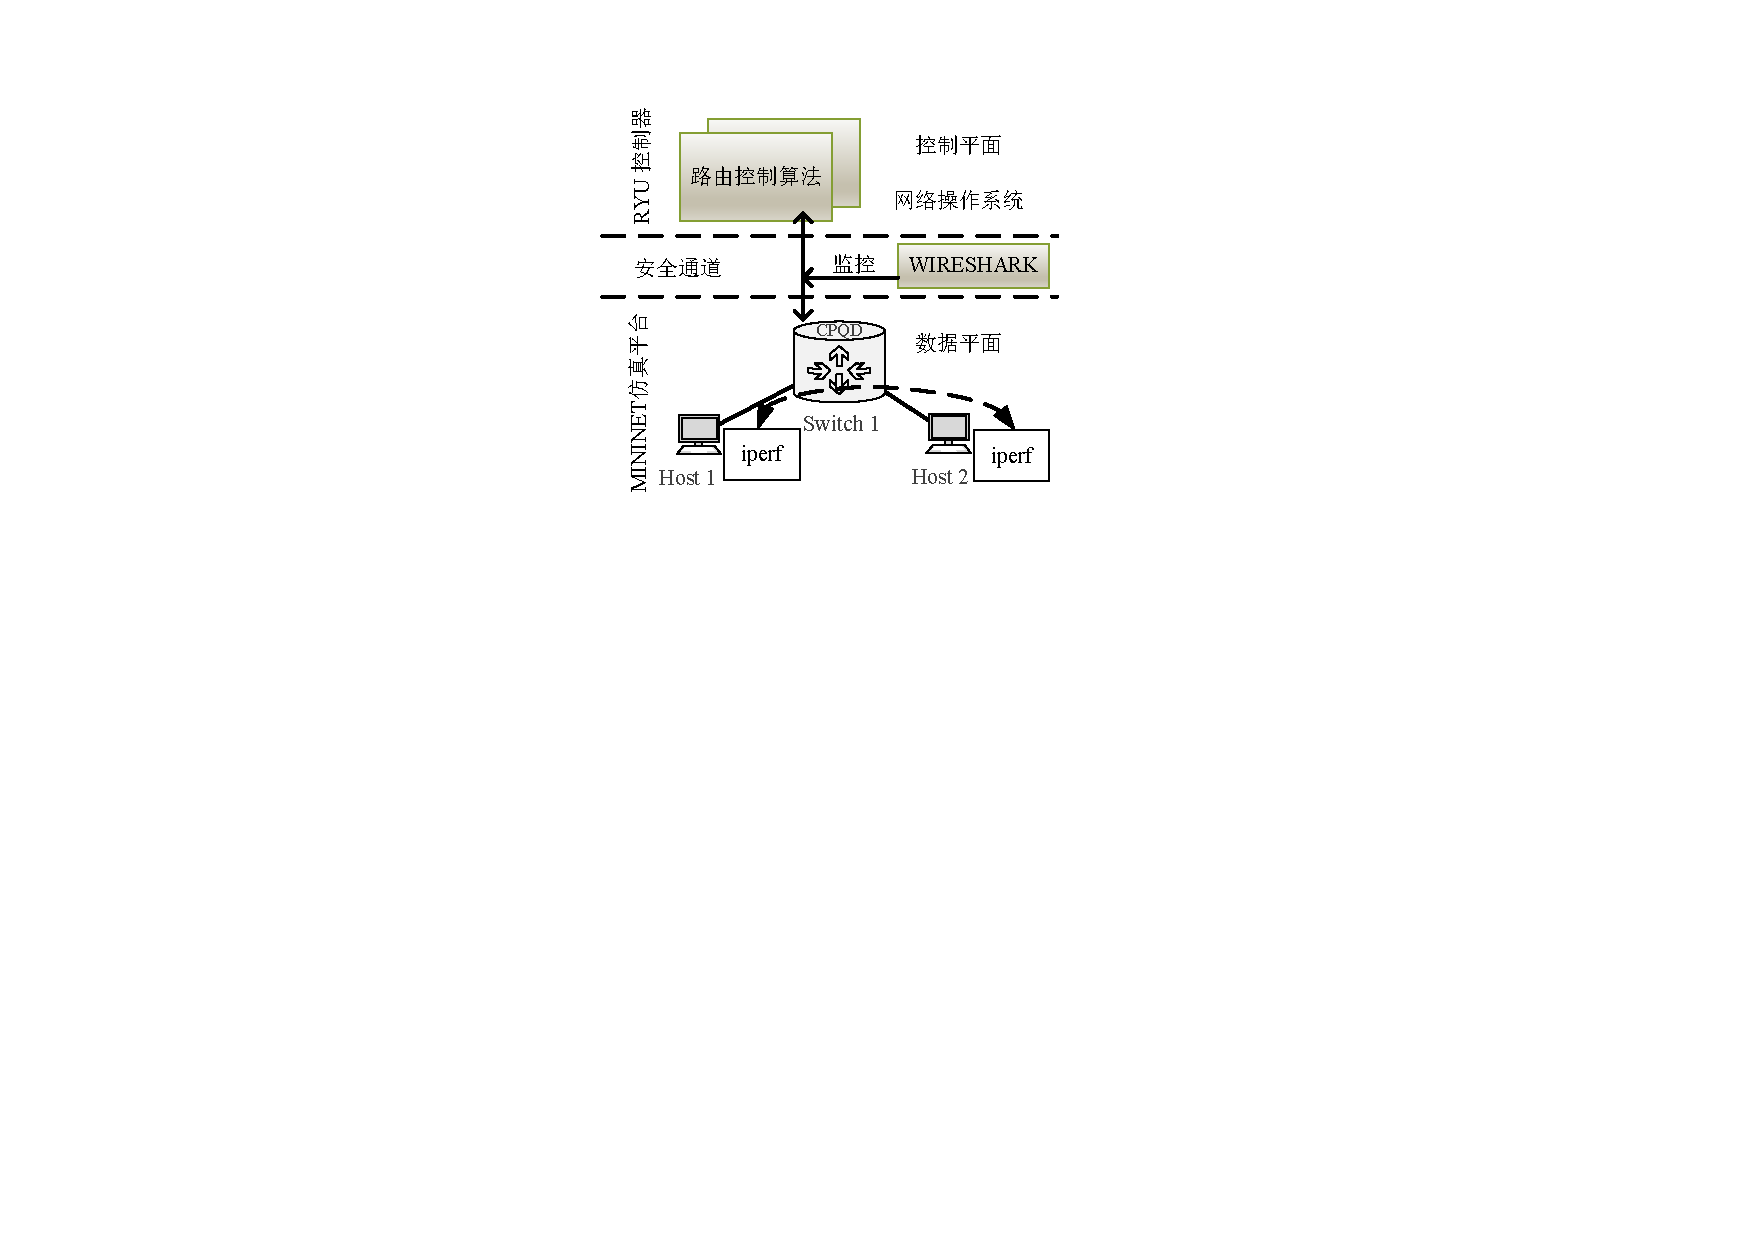
\includegraphics[scale=1]{ftsperf.pdf}
	\caption{性能测试实验拓扑} \label{fig:ftsperf}
\end{figure}

本文评估流表溢出对于通信速率和安全通道消息数量的影响,并且将之与使用FTS机制后的结果相比较。本实验平台使用x86服务器,Intel i3 CPU,8GB内存,ubuntu14.04,远端ryu控制器。实验拓扑如图\ref{fig:ftsperf}所示,性能测试中使用MININET[22]仿真工具建立单节点转发场景,使用iperf工具分别测试RTT和转发速率。利用wireshark工具分析安全通道内的控制消息数量。经过多次iperf流量测试后可到可信结果,当流表溢出时UDP传输有15\%的丢包率,TCP传输没有丢包。

\begin{figure}[!ht]
	\centering 
	\vspace{-1.5mm} 
	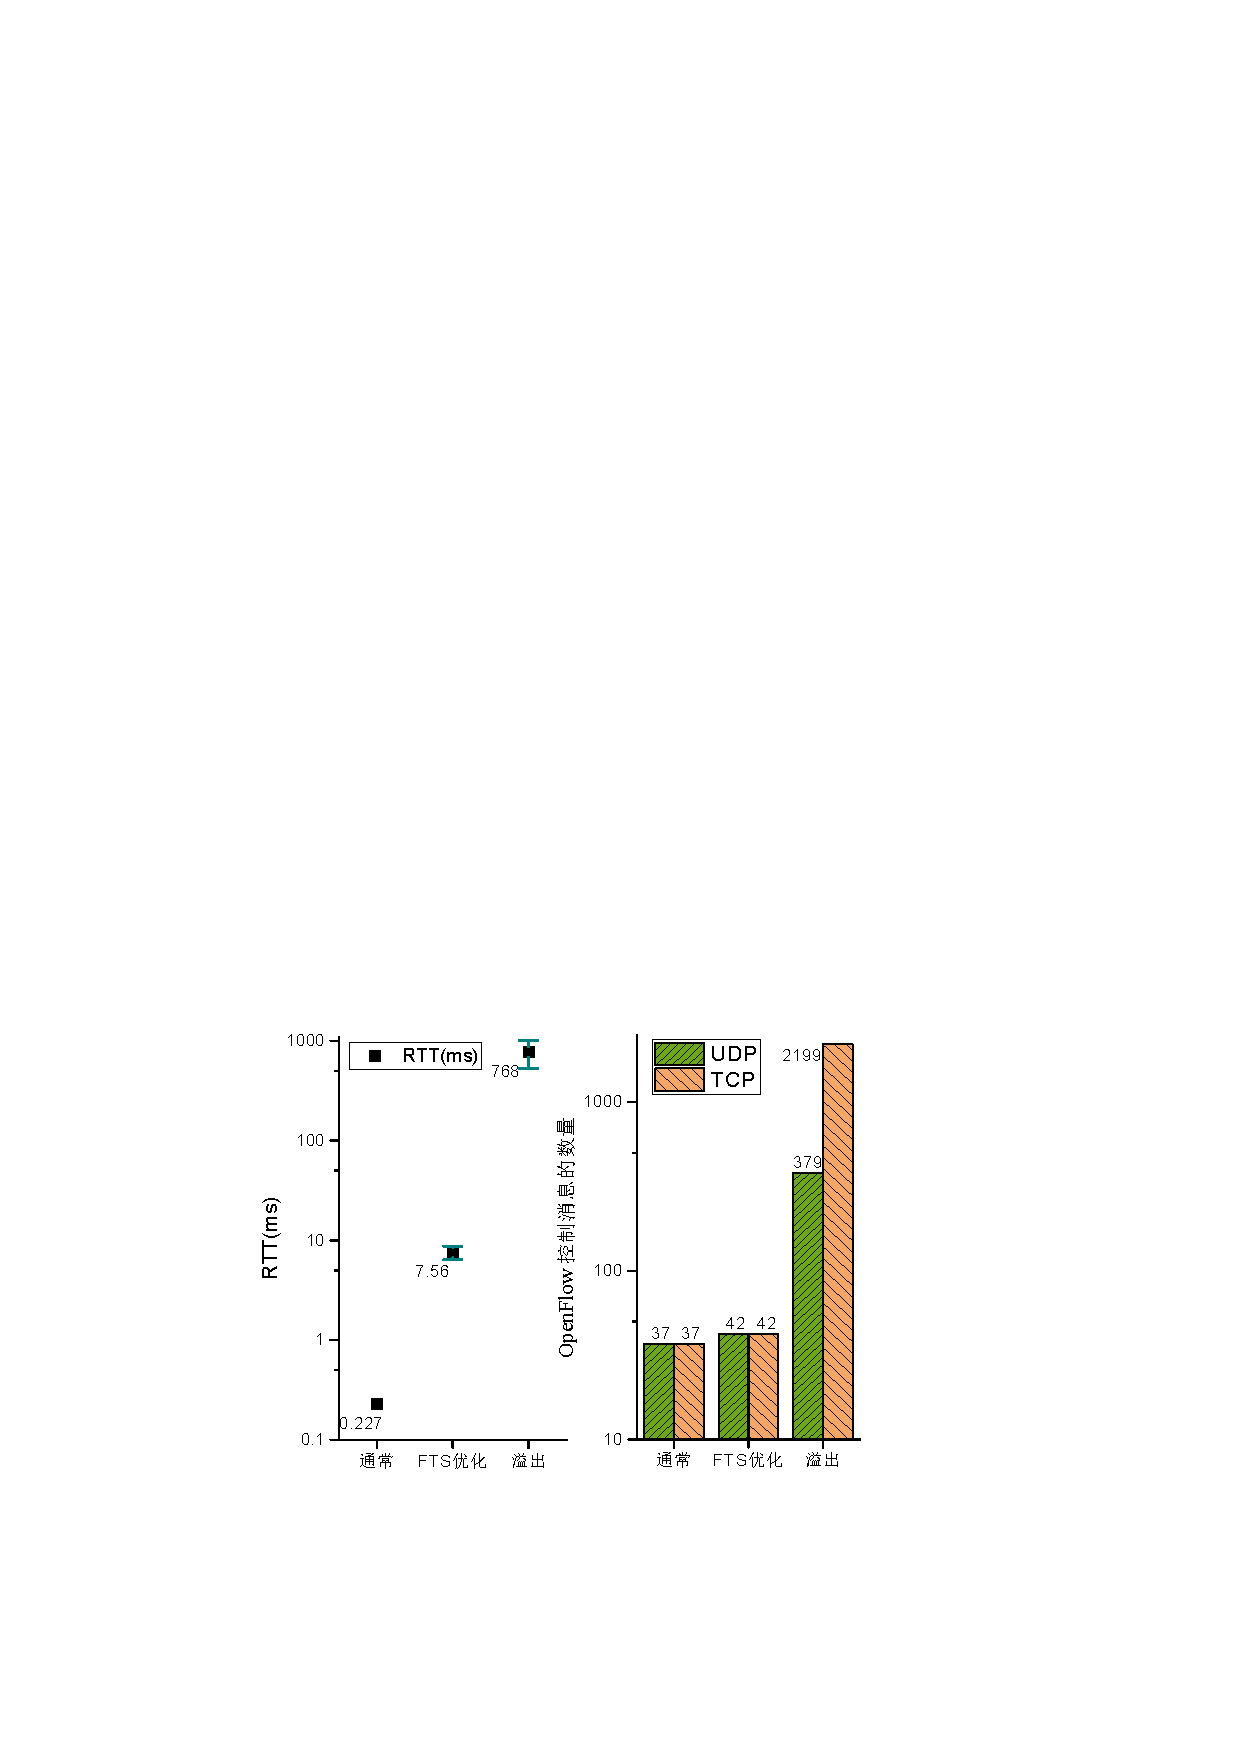
\includegraphics[scale=1]{ftsrtt.pdf}
	\caption{FTS与普通OpenFlow交换机再流表溢出时性能对比} \label{fig:ftsrtt}
\end{figure}

如图\ref{fig:ftsrtt}的右子图所示,当发生流表溢出时,建立UDP与TCP传输均消耗大量控制消息,比正常情况高出1到2个数量级。流表溢出导致既有表项被删除后重新下发原本流表信息,导致控制消息数目大量增加。而TCP传输消耗量大,可以通过TCP 的重传机制合理解释:TCP协议为保证所有包都到达过目的地,在发生丢包的情况下会重新发送数据包,这部分重传数据包对应着更多的控制信道数据。当交换机采用FTS策略时,当流表溢出时控制消息数量比正常情况多出13.5\%,相对最差情况提升了2个数量级。

如图\ref{fig:ftsrtt}的左子图所示,正常通信时数据包的转发平均时延为0.227ms,流表溢出时转发平均时延增加到768ms,通信时延比正常情况增加了4个数量级。这是因为流表溢出后正常转发的流表项会被删除,导致转发中断,重新安装流表项需要再次建立,耗费时间。因而导致总转发时延增大、吞吐率下降。同时可以看到,当使用FTS优化后,发生流表溢出后,转发延迟从768ms下降到8ms以内,同样优化了2个数量级。这是因为FTS机制在本地寻找其他转发路径并建立转发,可以大大降低控制器的冗余操作次数,并最多只需要消耗一次流表项的建立时间。

\BiSubsection{代价评估:额外消耗全局资源与流路径}{Overhead Evaluation} 

本小结测试,实施FTS机制后所需要的额外的转发资源。在流表容量限制下,建立非最短路径时额外增加的转发距离。

\begin{figure}[!ht]
	\centering 
	\vspace{-1.5mm} 
	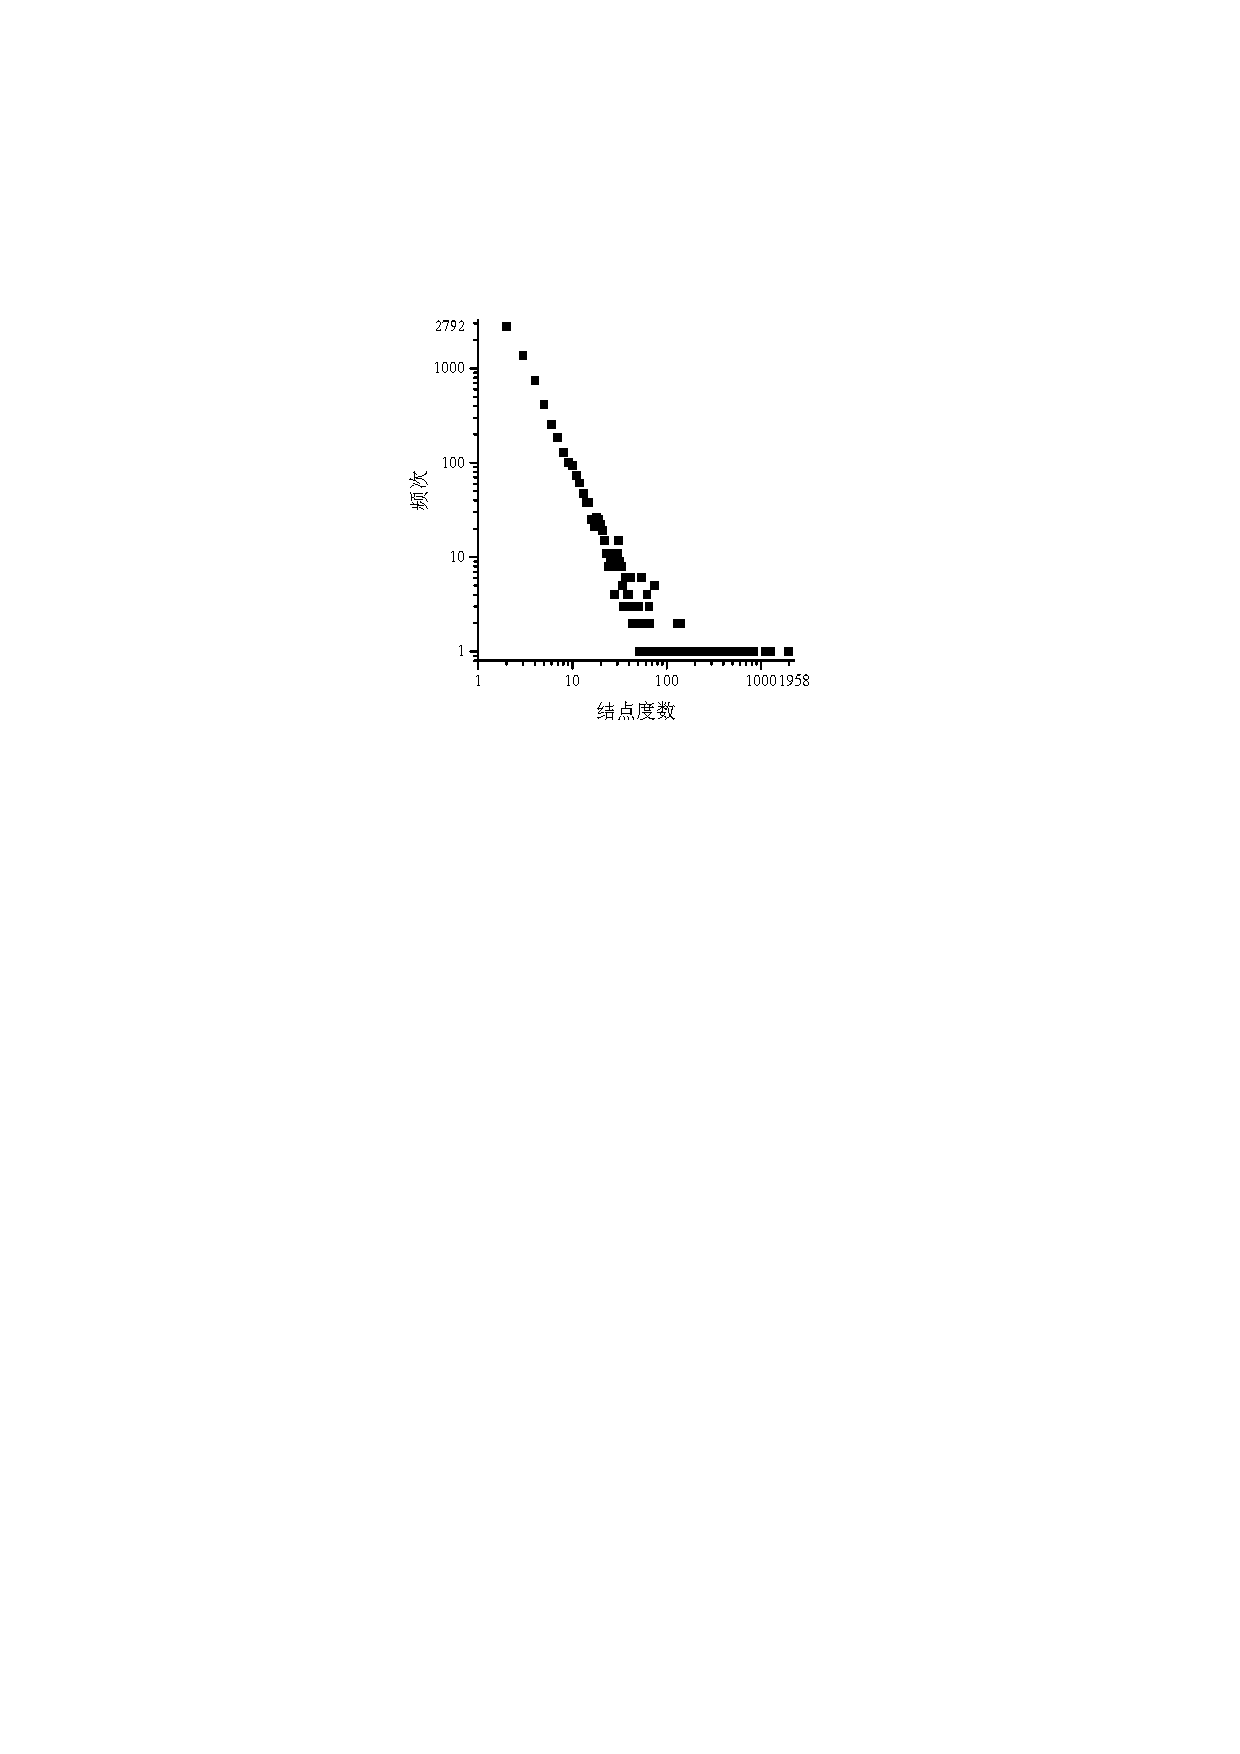
\includegraphics[scale=1]{ftsdu.pdf}
	\caption{实验用的真实拓扑结点度数特征分布} \label{fig:ftsdu}
\end{figure}

本文选取CAIDA公开的自治域真实拓扑\footnote{The CAIDA UCSD Macroscopic Skitter Topology Dataset  www.caida.org/tools/measurements/skitter <AS-level topology graphs > }数据,统计FTS机制下数据包到达目的地的总转发次数。在拓扑内共有6744个结点和26501条边,结点度数(每个节点的邻居交换机个数)分布可见图\ref{fig:ftsdu}。本实验将拓扑中的每个自治域抽象为一个转发节点,可以保留真实拓扑特征,也可以简化实验。

为减小流表溢出现象对交换机带来的副作用,FTS机制会使用邻居资源作为代价来完成正常转发。由于自主转发的随机性,到达目的地的路径并不一定是最短距离。本文计算了平均路径增加,路径总长度,路径长度与增加值的比例,以及额外总流表资源使用量。收到软件仿真工MININET的性能限制,多于数千个节点的仿真很难在其上完成。

第二个实验主要考察路由计算以及统计流表项数量,因而其实无需使用mininet完善的网络模拟功能,避免浪费实验的计算性能。本文使用C语言来提高仿真性能,实验只观察数据包的转发行为,以及转发节点的拓扑关系,忽略交换机的其他真实特性(例如,转发时延,端口,内部流水线等)。同时也忽略网络多层次结构(如,控制平面, 管道, 转发平面等),将网络抽象为理想的数学符号,网络功能只保留路由和FTS算法机制。

仿真网络的拓扑和功能简化后,还需要打入流量才能组成完整的实验。真实网络中流量巨大,链路数目多,端口连接复杂。本文做实验时无法得到完整的网络流量细节。其次即使得到所有流量状态信息,也不可能在仿真平台上再现真实网络情况。使用真实流量进行网络仿真时,一般需要专用的流量回放设备[23],需要专门的软硬件系统,不但造价昂贵,且实验复杂。网络连接中的每个端口都需要同时捕获流量。由于速率大,捕获设备只能保存短暂的场景。在测试时,只能针对单节点网络执行。用此方式完成全网仿真,无异于重新建设全部网络,显然不现实。因此本文计划直接通过逻辑推导得到统计值。

本文的基本思路如下:
1)流量仿真。生成拓扑内每个端口到端口的覆盖所有点对点的流,实现点点之间互联,流表信息是最完整的。
2)溢出仿真,假设仿真针对一个节点发生流表溢出时的场景。在这个流表溢出的节点,部署FTS算法。则可以分别得到向全部邻居节点随机转发后的网络状态结果。将得出的统计值归一化,来表示统计数据的概率密度。
此番假设仍有不足之处:本文假设网络中任意两点均可达并通信,但实际情况在同一时刻网络流量并不需要点点互达。
因此实验所表现的场景是网络拥堵时的较差情形。

通过实验本文只能得到变量统计值的平均概率密度,也是网络长时间运行后真实统计值的渐近线。然而面对庞大无的法完成的仿真任务,在实验精度上做取舍依然是值得且有效。

\begin{figure}[!ht]
	\centering 
	\vspace{-1.5mm} 
	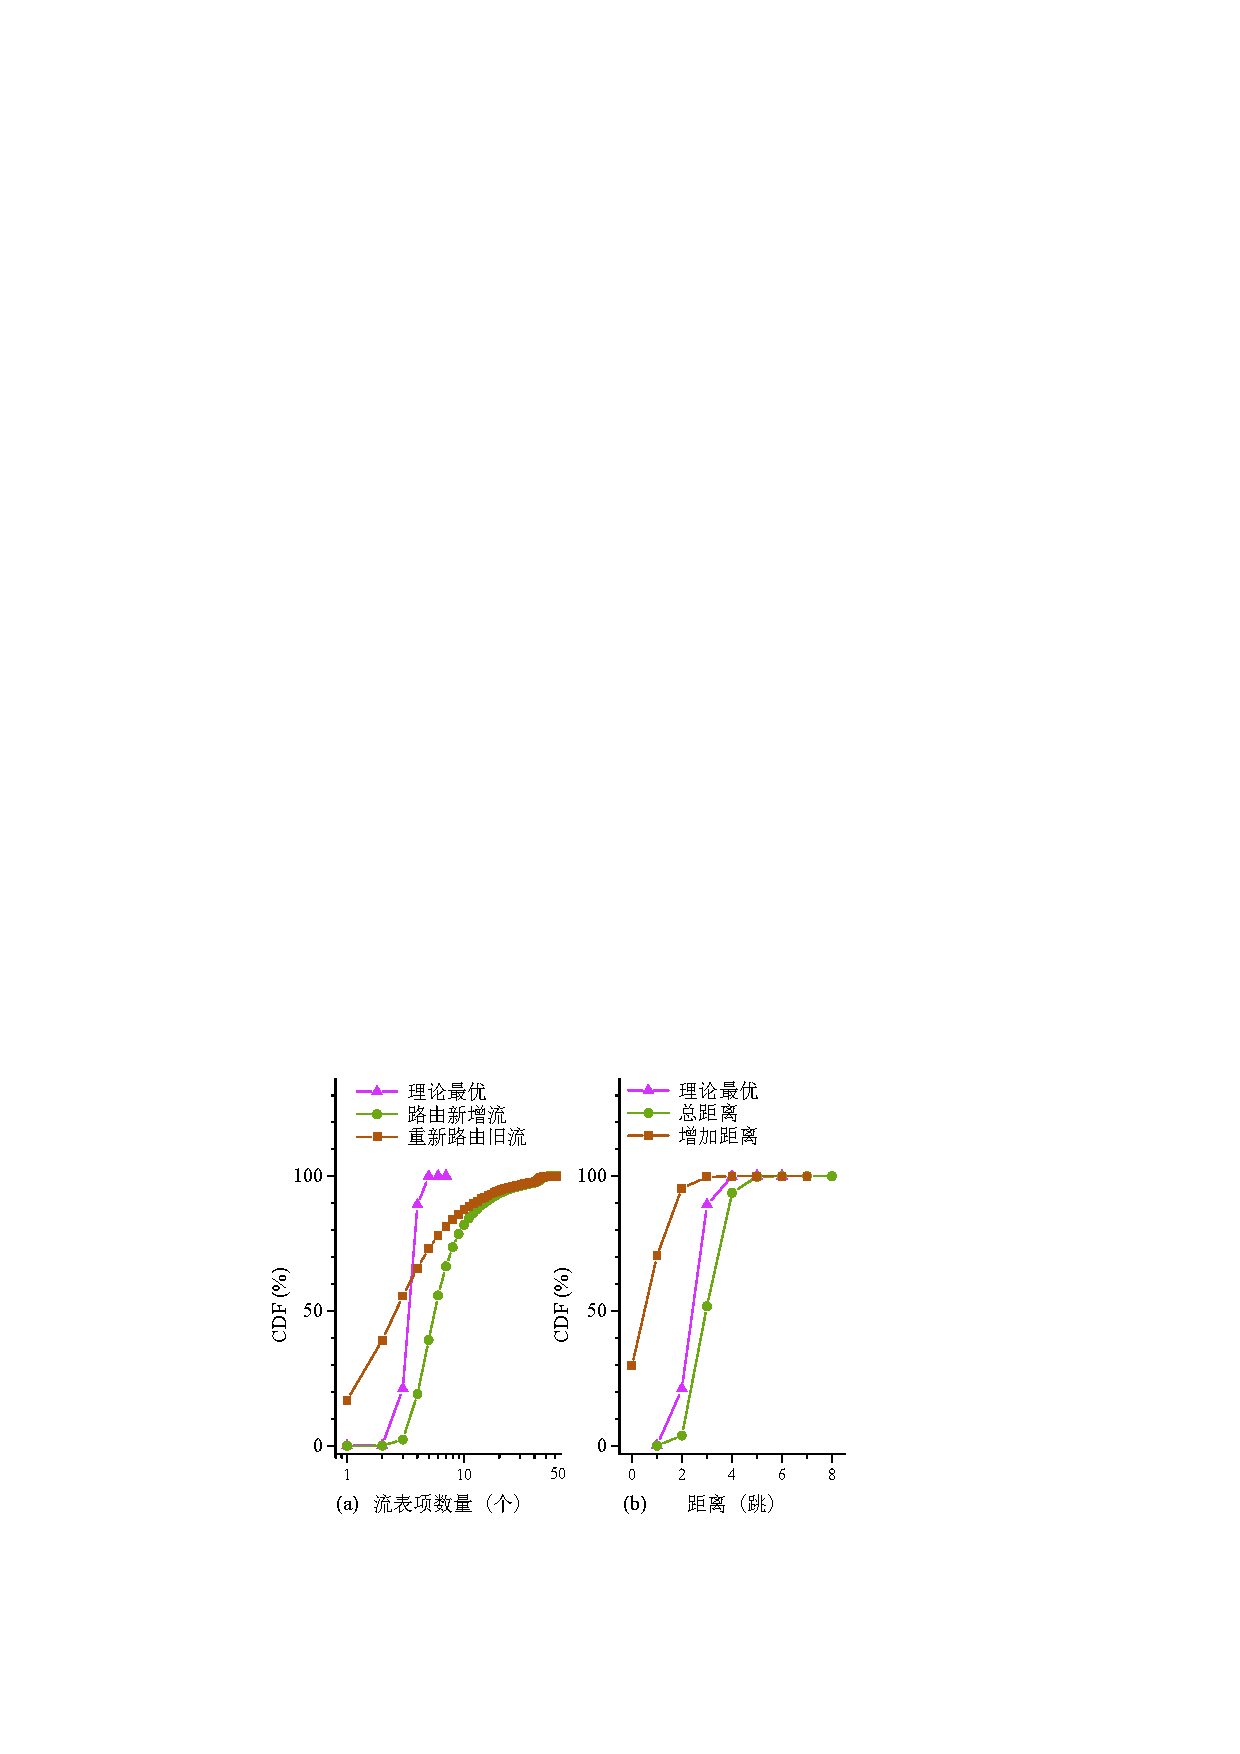
\includegraphics[scale=1]{ftsopt.pdf}
	\caption{当流表溢出时,FTS建立一条新流所消耗的额外流表项资源以及每个数据包从源到目的地的转发次数累计概率分布} \label{fig:ftsopt}
\end{figure}

图\ref{fig:ftsopt}(a)展示了FTS机制建立连接过程中使用的流表项数目的CDF曲线。由于FTS机制借用邻居交换机的流表项,流表资源总使用率与拓扑内节点平均邻居个数成正比。图中三角线段代表正常情况下流表的使用数量,圆形线段代表对新流实施FTS机制所需要流表项的数量,方块线条为正常流突然中断后使用FTS机制恢复通信所须的流表项数量。实验计算了激活FTS机制之后流表占用量的变化情况。因而方型线条表示某条活动的流被删除后FTS机制占用的流表总资源;圆形线条表示新流因流表溢出而无法建立连接的情况。前者平均须多占用流表5.9条,后者平均须多占用流表项8.7条。正常情况下新增流表项为3.9条。可以看出,在一个庞大的广域网中,FTS机制90\%概率下新增流表项不超过15条。99\%概率下新增流表项不超过45。最差情况为增加67条流表项。

图\ref{fig:ftsopt}(b)显示了FTS对数据包转发次数的影响。三角图线是正常情况下数据包的跳数。圆形图线表示FTS机制增加到达路径的平均长度。蓝色图线表示FTS机制中,流对比正常情况下多出的转发次数,可以看到95\%的概率FTS机制增加的跳数不会多于2跳。

\begin{figure}[!ht]
	\centering 
	\vspace{-1.5mm} 
	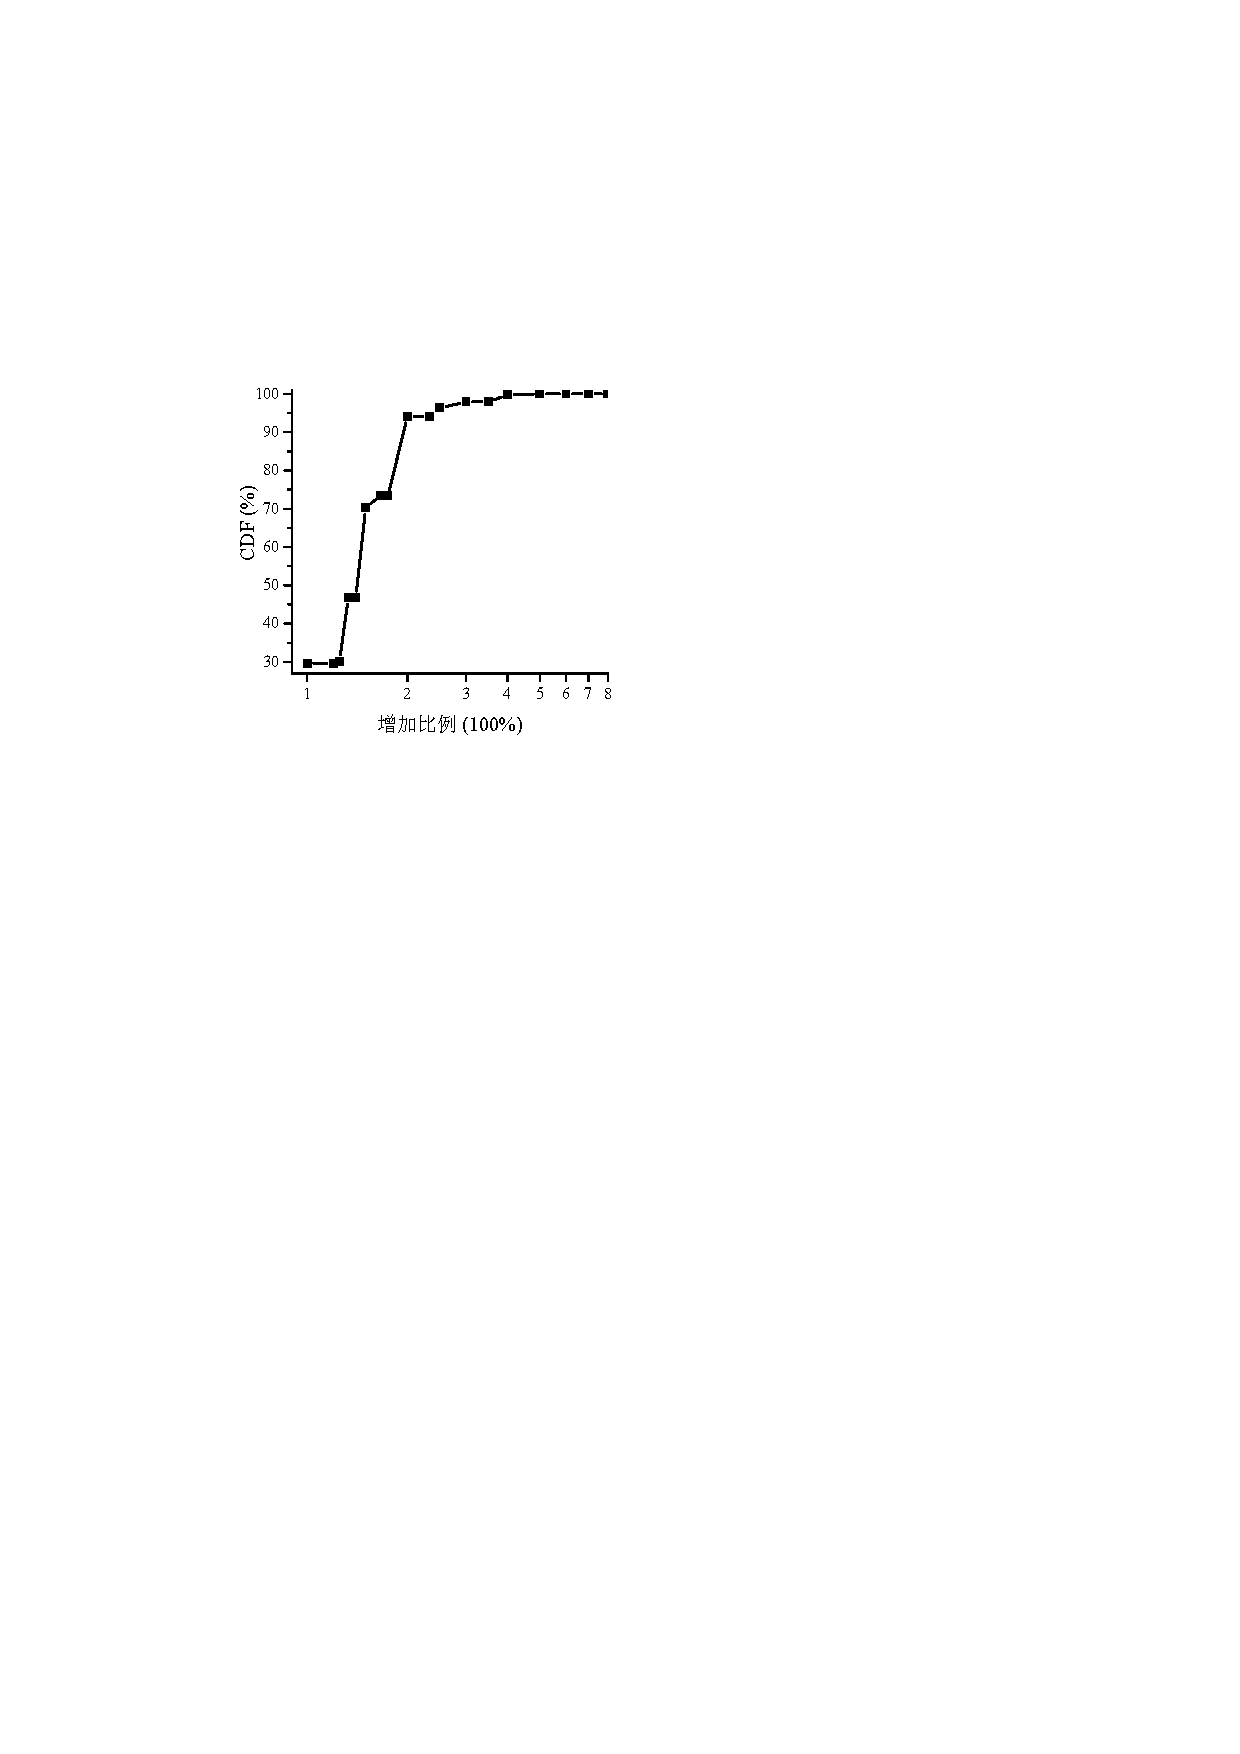
\includegraphics[scale=1]{ftsroute.pdf}
	\caption{相比最短路径,FTS完成路由增加的转发节点数量之比} \label{fig:ftsroute}
\end{figure}

图\ref{fig:ftsroute}示出FTS处理一条新流时,新流走过的路径的距离增长情况,在95\%的情形下路径增长不会达到最短路径距离的2倍。本文已将将仿真程序和拓扑数据、实验结果公开到github\footnote{https://github.com/qiaosiyi/test\_overflow\_random\_foward}上。



FTS不能保证同一TCP流量均往一邻居随机转发,并且数据包走过的路径长度也不尽相同。但是从图\ref{fig:ftsopt}(a)的实验结果得到:包包之间的路径差不超过7(8-1=7)跳。GE[24]网口标准转发时延为200us,因此总时间差不会超过2ms。这有可能启动TCP乱序重排机制,还有可能增加传输时延。但是,本文主要期望FTS机制能对流表溢出后的性能进行优化,并与流表溢出后转发设备的性能做对比,乱序导致的性能下降是可以忽略的。

\BiSection{本章小结}{Conclusion}

本章首先介绍了目前SDN架构中处理流量的方式,新兴的SDN、OpenFlow交换机是学术界研究的热点。在\ref{chap53}小节通过流量特征分析流表溢出的危害性以及不可避免性,相比于传统的网络交换设备,OpenFlow交换机需要消耗更大的查找表容量,流表溢出带来的性能下降现象较为严重。本文基于流量分布规律以及理论分析,在第\ref{chap54}小节提出基于全局资源的流表共享优化机制,扩展了OpenFlow交换机的Table-Miss处理方式。可以有效地缓解流表溢出现象带来的巨大网络通信性能损失。

第\ref{chap55}小节探讨了方案可执行性已经实现方法,最后本文在第\ref{chapftsevaluation}小节本文评估并证明了本文的方法可有效缓解流表溢出所带来的危害。文中从两方面验证了FTS机制,从实验结果中可以得出FTS机制有以下三个优点:(1)当流表溢出时,FTS相比于目前的Table-Miss处理模式可有效地降低控制消息数量和RTT时延达两个数量级。(2)本文提出了一种有效的快速外部组表选择算法。(3)FTS易于在真实交换机上部署和控制,占用硬件资源少,与现行Table-Miss处理模式兼容。

转发设备硬件资源消耗量大以及设备成本高是目前SDN网络向广域网推进的重要难点。其中流表资源的匮乏有是该问题的核心点,本文提出的FTS机制将为后续SDN发展提供一个可参考的容错机制。






